\chapter{Building Envelope Thermal Optimisation using Computer Algorithm}

\paragraph{Introduction of Algorithmic Input to the Design Proces\mbox{}\vspace{-0.3cm}s}\mbox{}

An important issue to be considered is the point at which algorithm is introduced to the design process. The introduction of algorithm (and simulation for that matter) at a very early stage as opposed to at a point when the schematic design has been almost finished would greatly influence the final product; as the former is considered pure form generation governed by optimisation algorithms, while the latter is considered optimisation of a geometry which has already been defined by the architect, and in turn defining the major optimisable variables.

Although the above would suggest that algorithmic form generation is best introduced at the earliest stage possible, this is not practical, as it would mean that endless possibilities can be explored with no regard to user requirements. Therefore, for the sake of simplicity and practicality, it has been assumed that a conceptual form has been designed and used as a basis for further algorithmic optimisation. Form generation in this case is mostly \emph{regeneration} of the modelled geometry representing the building envelope.

\section{Stages of Building Envelope Thermal Optimisation}

The information presented so far requires at this point that a clear methodology, properly sequenced, and categorised, formulated out of the concepts and tools illustrated so far in the thesis.

To recapitulate the purpose of the thesis; the aim is to provide a practical method, sufficiently supported by previous experimentation, of designing a building envelope which meets the thermal performance criteria of the designer, through iterative environmental simulation and algorithmic optimisation, algorithmic form generation and regeneration.

The proposed procedure to guide such and endeavour, is based on the elements of the process described in the previous chapters, but differs in sequence to suite the natural order of the design process, and is as follows:

\begin{enumerate}
	\item Analysis of Envelope Form
	\item Design Intent: Thermal Criteria and Target Performance
	\item Virtual Modelling and Simulation
	\item Programming and Optimisation
\end{enumerate}

The above stated stages will be presented in the form of general guidlines and important notes for the architect to consider, and will also act as key for the reader to all relevant sections of the thesis. Afterwards, a more detailed case-by-case description of the procedure and the underlying concepts will be provided, with examples of worked out envelopes (see section \ref{sec:DetailedProcedure}).

\clearpage
\colorbox{95Gray}{%
	\begin{minipage}[c][20.5cm][t]{\textwidth}{%
		\subsection{Stage 1: Analysis of Envelope Form}
		\label{sec:Stage1}
		\vspace{0.5cm}
		\begin{enumerate}
			\item \textbf{Develop an initial schematic/conceptual design}\footnote{Additional information on development of architectural form can be found in publications such as \emph{Architecture: Design Notebook} \cite{fawcett03}.}
				\begin{itemize}
					\item Analysing the context and responsiveness to building site and conditions
					\item Developing the initial building image and type
					\item Choosing the appropriate technologies (structural)
					\item Finalising the conceptual envelope form to include opening, architectural features in elevations, roof form\ldots etc.
				\end{itemize}
			\vspace{0.2cm}
			\item \textbf{Assign the developed building form under a predefined category of envelopes}\\[3mm]
				The category of building envelope will have implications in the determination of thermal control mechanisms. The process of envelope categorisation has been discussed at length in section \ref{sec:AnalyseEnvelope}.
		\end{enumerate}
		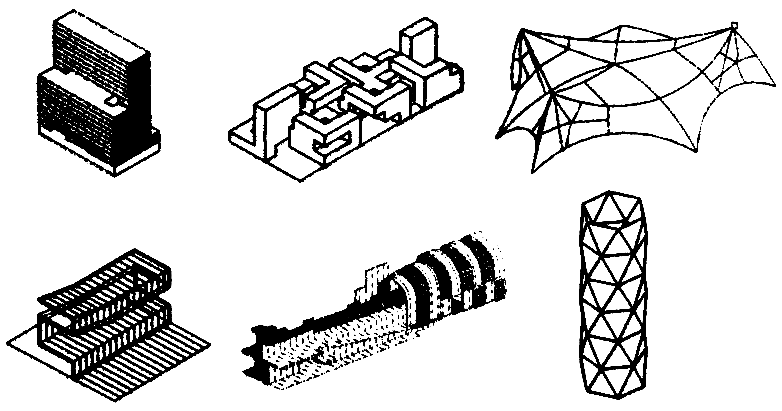
\includegraphics[width=\textwidth]{./Images/23-StageA}
		\begin{center}
		\small A number of different building envelope forms
		\end{center}
	}%
\end{minipage}%
}

\clearpage
\colorbox{95Gray}{%
	\begin{minipage}[c][20.5cm][t]{\textwidth}{%
		\subsection{Stage 2: Design Intent - Thermal Criteria and Target Performance}
		\label{sec:Stage2}
		\vspace{0.5cm}
		\begin{enumerate}
			\item \textbf{Assign thermal performance targets at different reference points/internal spaces}\\[3mm]
				Based on the requirements of the building and the internal space functions, the architect should assign the target temperature levels. These values will act as an important input to the optimisation algorithm (for a reference on thermal comfort, refer to section \ref{sec:ThermalComfort}).\\[3mm]
				\textbf{Note:} The target temperature levels referenced herein are controlled by passive solar control techniques. Any additional concerns such as HVAC loads are to be considered after the optimisation.
			\item \textbf{Determining the Thermal Control Mechanism}\\[3mm]
				Depending on the category of building envelope, the most effective control mechanism will be chosen for optimisation. The scope of this thesis is focused on passive solar control mechanisms which include:
				\begin{enumerate}
					\item Shape
						\begin{enumerate}
							\item Surface-to-volume Ratio
							\item Orientation
						\end{enumerate}
					\item Fabric
						\begin{enumerate}
							\item Shading
							\item Surface Material Properties
						\end{enumerate}
					\item Fenestration
						\begin{enumerate}
							\item Size, Position and Orientation
							\item Glazing Material
							\item Closing Mechanism
							\item External Shading
						\end{enumerate}
				\end{enumerate}
				These control mechanisms are discussed at length in sections \ref{sec:ThermalDesignVariables} and \ref{sec:DesignIntent:Thermal}.
		\end{enumerate}
	}%
\end{minipage}%
}


\clearpage
\colorbox{95Gray}{%
	\begin{minipage}[c][20.5cm][t]{\textwidth}{%
		\subsection{Stage 3: Virtual Modelling and Simulation}
		\label{sec:Stage3}
		\vspace{0.5cm}
		\begin{enumerate} \item \textbf{Creating the 3D Parametric Model}\\[3mm] It is of the utmost importance that the building 3D model be parametric. If the building is modelled in a CAD programme that does not recognize the objects as smart objects with predefined parameters, the optimisation of the building envelope cannot be performed (refer to section \ref{sec:GeoModel} for reference on building geometry breakdown into procedures and parameters).\\

				Examples of programmes capable of parametric modelling:
				\begin{enumerate}
					\item Parametric modelling environments such as \textsc{catia} or Rhinoceros/Grasshopper (see Chapter 4).
					\item Direct modelling into simulation environemnts with GUI's and visualisation capabilities such as \textsc{ecotect} (refer to section \ref{sec:SimulationPrograms}). This is the most preferred as it would allow scripting (see Stage 4, point no. 1).
					\item Creating the building model in a BIM [Building Information Modelling] environment.
				\end{enumerate}
				\vspace{0.2cm}
			\item \textbf{Simulation of the Building Model}\\[3mm]
				Selecting the simulation programme is based on the control mechanism of thermal performance as decided earlier in stage 2. A large number of simulation programmes have been discused at length in section \ref{sec:SimulationPrograms}. Other factors are also explained in section \ref{sec:SimulationModel}.\\
				Popular simulation environments include:
				\begin{enumerate}
					\item \textsc{ecotect} (see page \pageref{par:ECOTECT})
					\item \textsc{EnergyPlus} (see page \pageref{par:EnergyPlus})
					\item \textsc{doe-2.1e} (see page \pageref{par:DOE})
					\item e\textsc{Quest} (see page \pageref{par:eQUEST})
					\item \textsc{transys} (see page \pageref{par:TRANSYS})\\
						\ldots among others
				\end{enumerate}
		\end{enumerate}
	}%
\end{minipage}%
}

\clearpage
\colorbox{95Gray}{%
	\begin{minipage}[c][20.5cm][t]{\textwidth}{%
		\subsection{Stage 4: Programming and Optimisation}
		\label{sec:Stage4}
		\vspace{0.5cm}
		\begin{enumerate}
			\item \textbf{Determine the Programming Method}\\[3mm]
				The architect must determine at this stage the method of programming the algorithm to optimise the building performance. \textbf{Note:} the process of optimisation can be very frustrating to the architect if this stage is not planned well. There are two main possibilities for the programming method:
				\begin{enumerate}
					\item \textbf{The simulation programme supports scripting} (refer to section \ref{sec:EndUserProgramming} for End-User Programming or \emph{Scripting}). In this case the algorithm can be programmed directly into the simulation programme.
					\item \textbf{The simulation programme does not support scripting}
						\begin{enumerate}
							\item Programme the algorihm in a language such as \textsc{Java} or C$++$ 
							\item Exchange of temperature values, and building parameter values between the algorithm, simulation environment, and parametric modelling programme.
						\end{enumerate}
				\end{enumerate}
			\item \textbf{Choose the Optimisation Algorithm}
				\begin{enumerate}
					\item \textbf{Genetic Algorithm:} Creates a \emph{set} of final solutions, giving the architect the advantage of choice.
					\item \textbf{Simmulated Annealing:} Focuses on findng the global optimum.
					\item \textbf{Tabu Search:} Can handle very large solution spaces or complex problems.
				\end{enumerate}
			\item \textbf{Initiate Optimisation and Simulation}\\[3mm]
				The optimisation algorithm is now programmed, and the virtual model parameters are optimised through the algorithm and each individual solution is assessed by simulation.
			\item \textbf{Termination Conditions Met}\\[3mm]
				At this point the target values of the design intent have been met and the optimisation algorithm can terminate and present the final results.
		\end{enumerate}
	}%
\end{minipage}%
}

\section{Context, Underlying Concepts and Detailed Procedure}
\label{sec:DetailedProcedure}

\subsection{Analysis of Envelope Form}
\label{sec:AnalyseEnvelope}

As described earlier, any building envelope is composed of the architectural physical elements that separate the inside from the outside, creating an \emph{envelope} or \emph{enclosure} for the building (see page \pageref{BuildEnvDef}).

Although this definition applies to almost all building envelopes, they would vary greatly from one building to another, making the task at hand; which is the utilisation of algorithmic design and thermal simulation to achieve thermally efficient buildings, inefficient or even practically meaningless, unless proper categorisation of building envelope design is made.

This is due to the fact that with differences between building enclosure designs, the variables that affect the thermal performance of the envelope will have varying degrees of impact, sometimes even reaching almost zero impact in some cases; therfore, it essential that the architect determines which variable should be given the priority over others.

\paragraph{Categorisation of Building Envelopes}\mbox{}

One interesting way of categorising building enclosures, is the endeavour undertaken by the \emph{Foreign Office Architects} to categorise their own work in a book named \emph{Phylogenesis: FOA's Ark} \cite{foa04}. The categorisation system resembles a biological evolutionary tree, that starts from one point and branches into different species through several evolutionary stages (figures \ref{fig:Phylogenesis} and \ref{fig:FOAEnvelopes}).

The categorisation of building envelopes used by the Foreign Office Architects provides a good example for analysis of different envelope forms and assigning them under a building category. This categorisation method is used as a basis for the examples given at the end of the chapter; however, the particular method of categorisation presented in Phylogenesis does not correspond directly to thermal design variables of building envelopes, and further analysis of each species or category is needed to determine the significance of each aspect of the form from a thermal point of view.

According to the previously mentioned evolutionary tree of building forms, the building envelopes were categorised in the following manner:

\setlength{\columnseprule}{1pt}
\begin{multicols}{2}
\begin{enumerate}
	\item \textbf{Function}\\
		The predominant function of the surface.
		\begin{enumerate}
		\item Ground
		\item Envelope
		\end{enumerate}
	\item \textbf{Faciality}\\
		How many faces/layers the surface divides space into.	
		\begin{enumerate}
			\item Single Face (the ground)
			\item Multiple Face (a slab with flooring and ceiling on each side)
		\end{enumerate}
	\item \textbf{Balance}\\
		The relationship between the surface and gravity.
		\begin{enumerate}
			\item Constant
				\begin{enumerate}
					\item Perpendicular (roof or ground)
					\item Parallel (wall)
				\end{enumerate}
			\item Shifting (blob or shed; i.e. continuously moving from perpendicular to parallel)
		\end{enumerate}
	\item \textbf{Discontinuity}\\
		The amount of interruptions/alteration to the continuous surface.
		\begin{enumerate}
			\item Planar (no interruptions)
			\item Rippled (small interruptions)
			\item Pinched (highly accentuated interruptions)
			\item Perforated (local interruptions)
			\item Bifurcated (interruptions extending to other layers of space)
		\end{enumerate}
	\item \textbf{Orientation}\\
		Spacial ordering of singularities, i.e. pattern
		\begin{enumerate}
			\item Oriented
				\begin{enumerate}
					\item Striated (parallel order)
					\item Polar (respond to poles/centres)
				\end{enumerate}
			\item Non-oriented (no detectable pattern)
		\end{enumerate}
	\item \textbf{Geometry}\\
		Continuouity of surfaces.
		\begin{enumerate}
			\item Continuous (smooth)
			\item Discontinuous (broken with edges)
		\end{enumerate}
	\item \textbf{Diversification}
		\begin{enumerate}
			\item Patterned
			\item Contingent
		\end{enumerate}
\end{enumerate}
\end{multicols}

\begin{sidewaysfigure}[htbp]
	\centering
	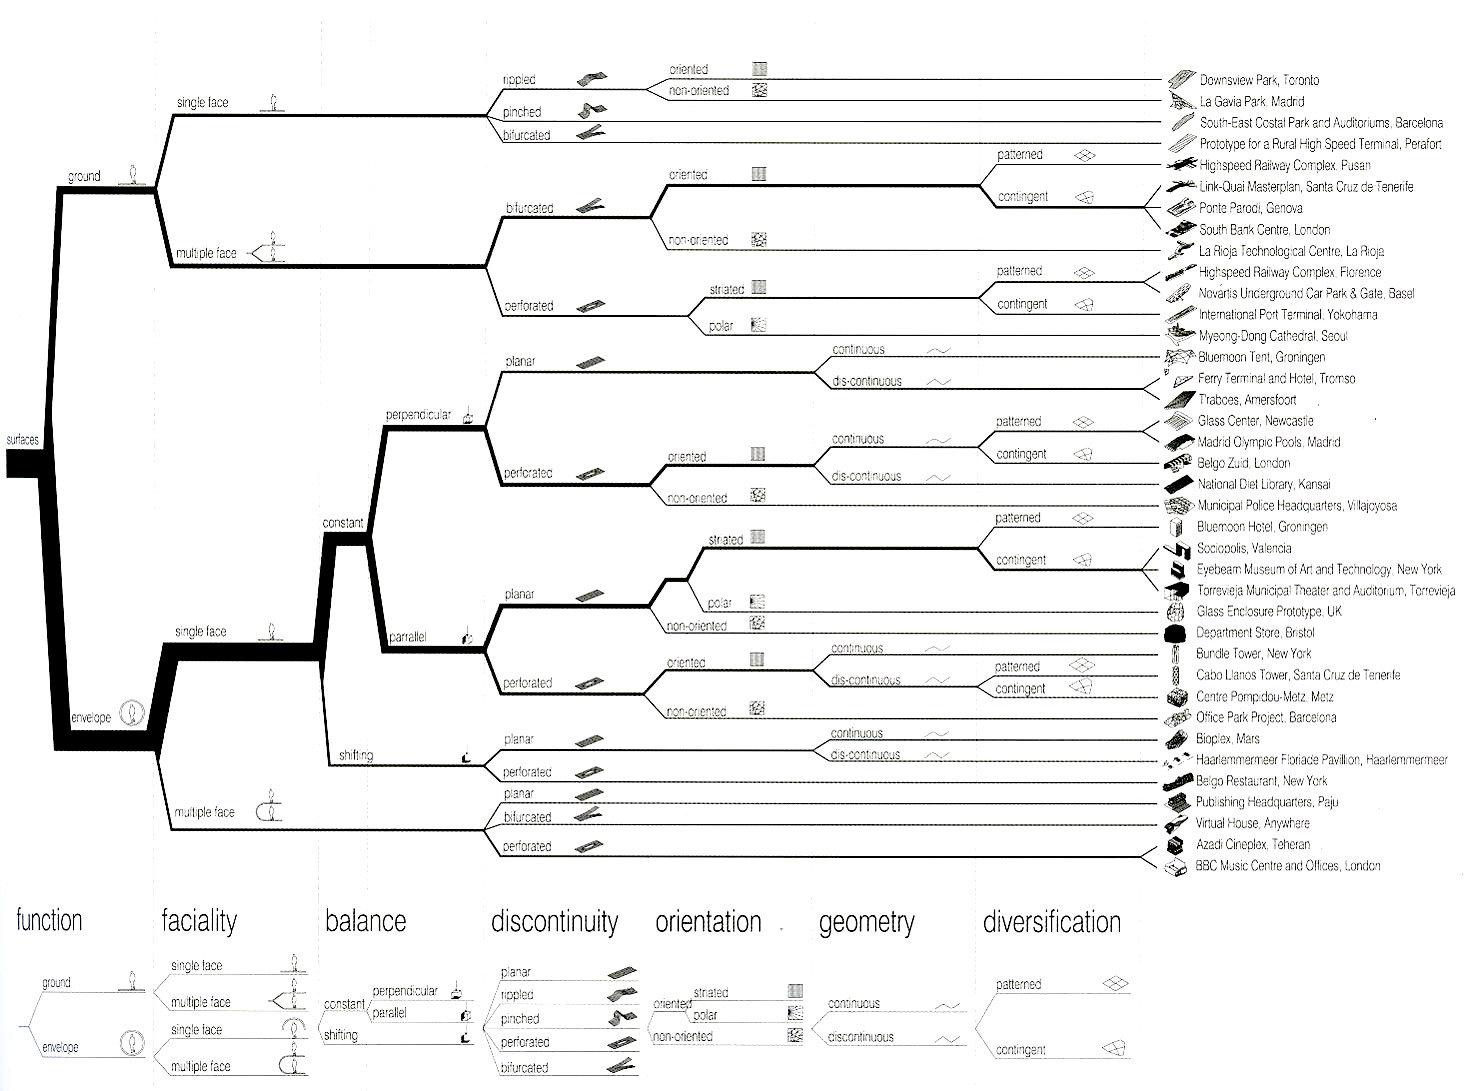
\includegraphics[width=20cm]{./Images/1-Phylogenesis}
	\caption[FOA Phylogenesis]{Structures Categorisation of FOA Work, Including Envelope Categorisation According to \emph{Phylogenesis} \cite{foa04}}
	\label{fig:Phylogenesis}
\end{sidewaysfigure}

\begin{figure}[H]
	\centering
	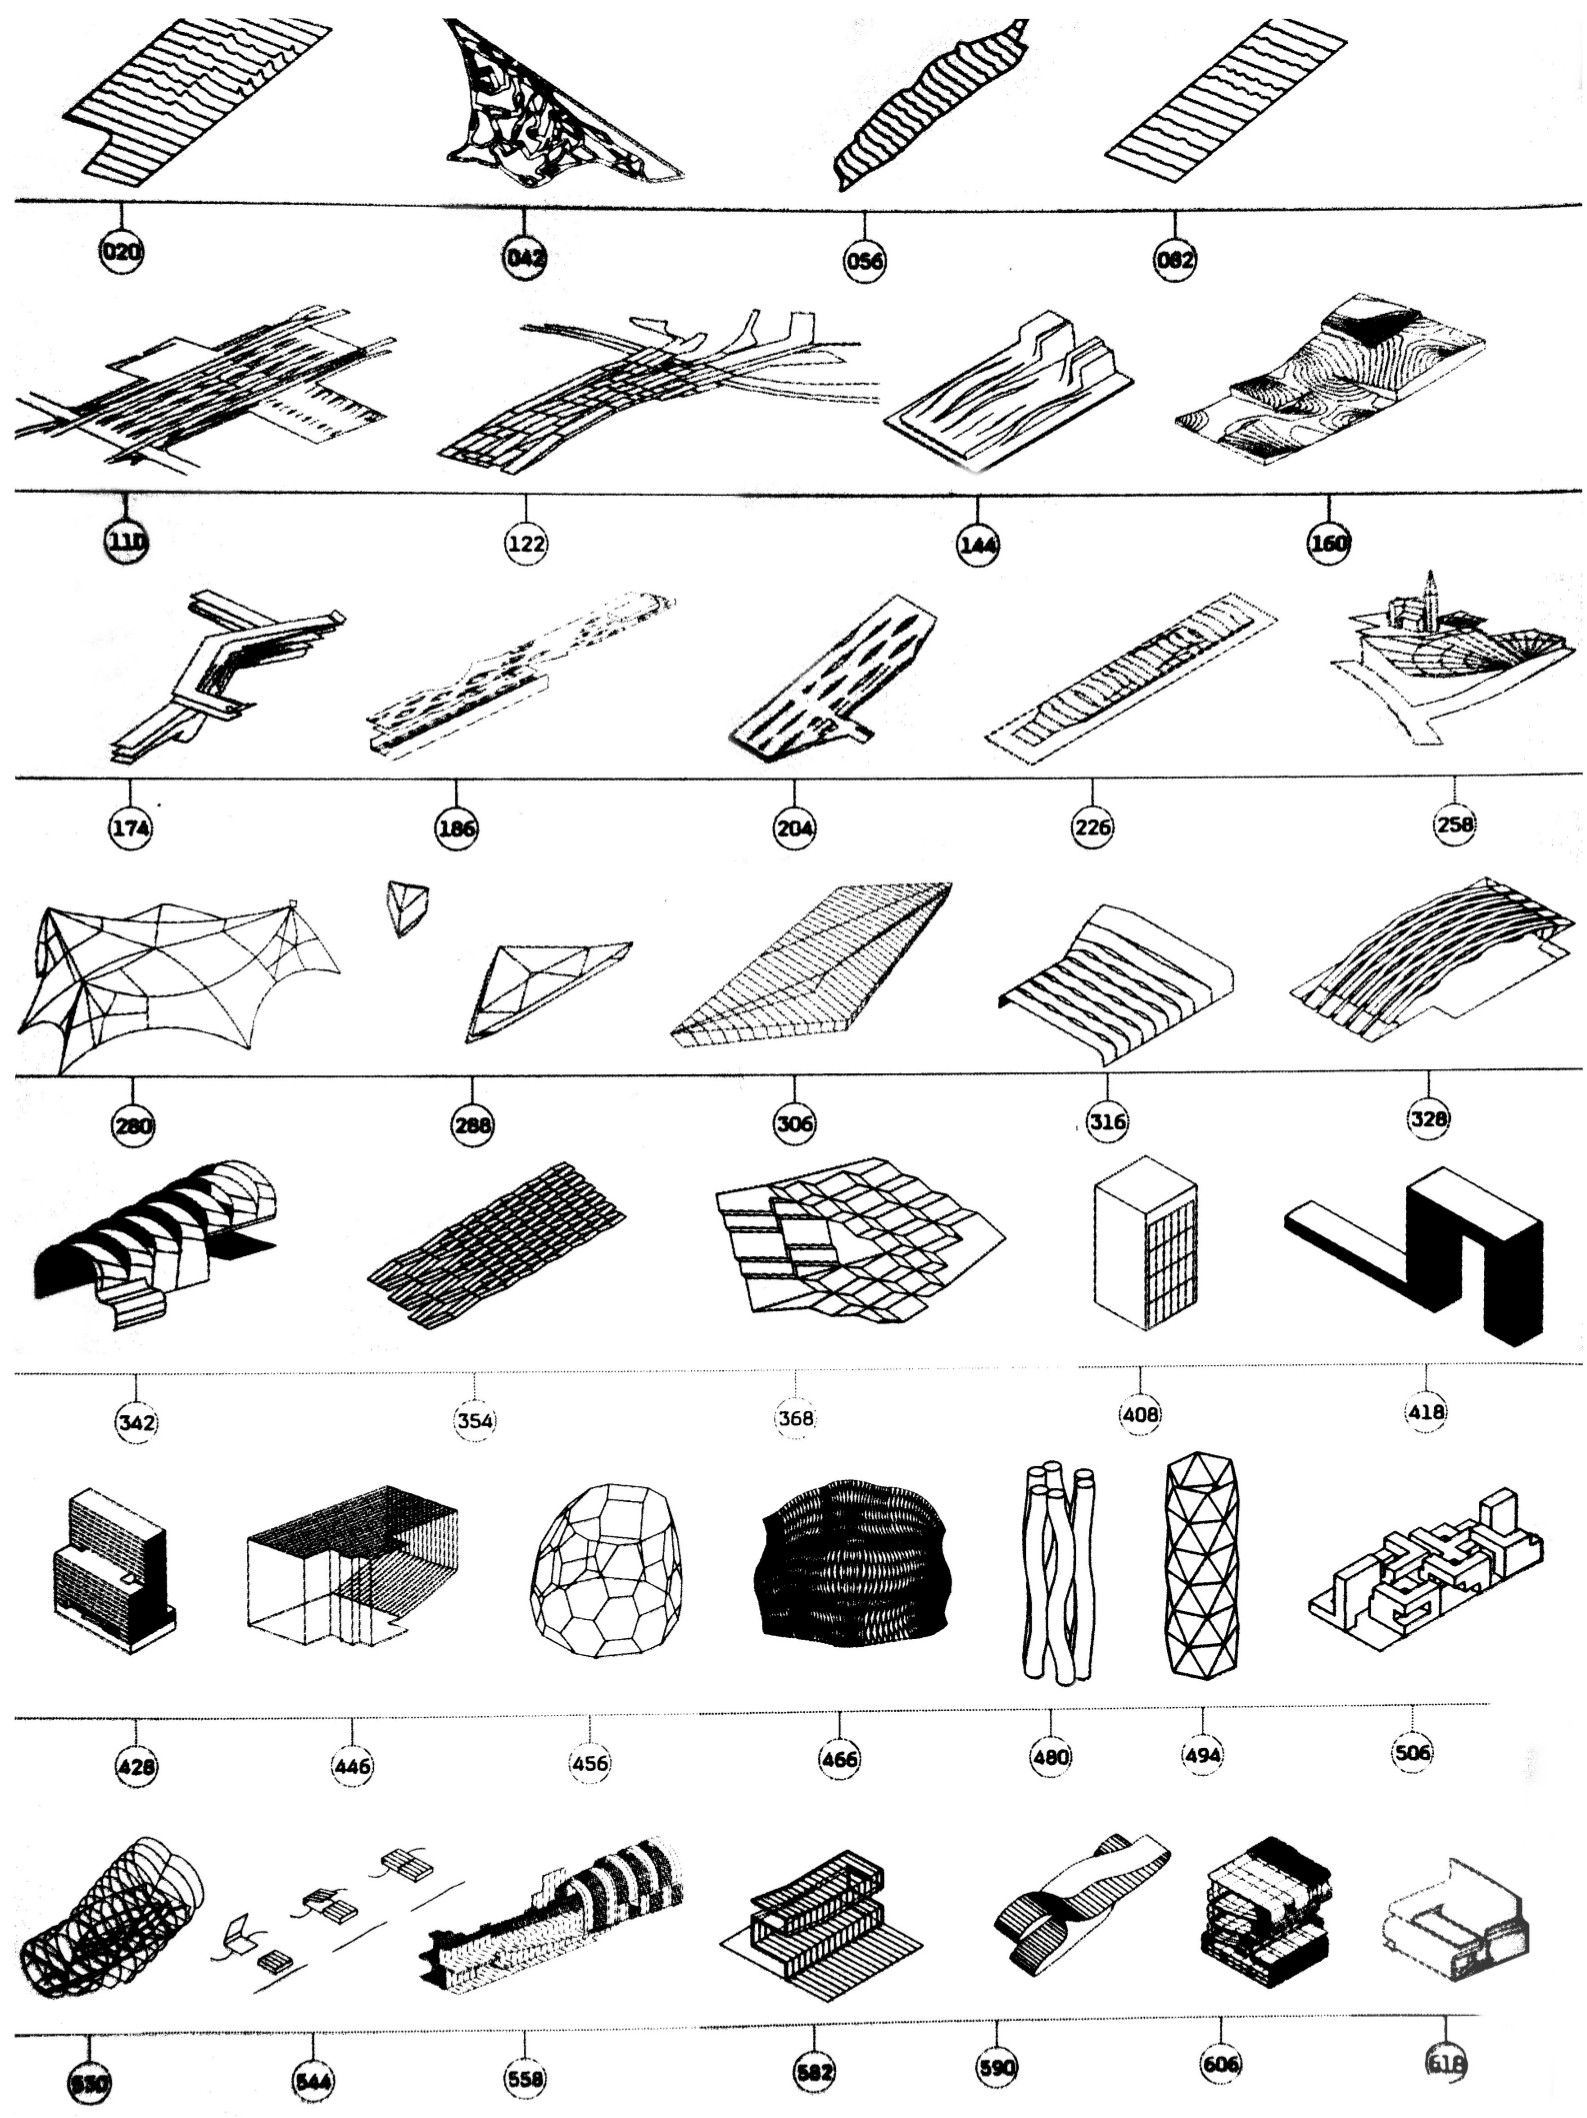
\includegraphics[width=\textwidth]{./Images/2-Envelopes}
	\caption[FOA Building Envelopes]{Examples of Structures and Building Envelopes by FOA \cite{foa04}}
	\label{fig:FOAEnvelopes}
\end{figure}

\clearpage
\subsection{Design Intent: Thermal Criteria and Target Performance}
\label{sec:DesignIntent:Thermal}

Having created a system of categorisation in which any envelope form can mostly fit under a category; the thermal design through algorithm and simulation should be guided by the variables that affect the particular envelope form the most.

Here we refer to the design variables listed earlier in Chapter 3 (see page \pageref{sec:ThermalDesignVariables}), which are concerned with thermal design through passive solar control. This holds true in Chapter 4 as well, and has been done as such with the intention of simplifying the process and narrowing the scope for easier but effective illustration of the concepts throughout the thesis.

For the sake of convenience, the variables are re-listed here in table form.

\begin{table}[H]
	\centering
	\begin{tabular}{l|l}
		\textbf{Shape}		&Surface-to-Volume Ratio\\
					&Orientation\\
					&\\
		\textbf{Fabric} 	&Shading\\
					&Surface Material Properties\\
					&\\
		\textbf{Fenestration}	&Size, Position and Orientation\\
					&Glazing Material\\
					&Closing Mechanism\\
					&External Shading\\
	\end{tabular}
	\caption{Thermal Design Variables}
	\label{tab:ThermalDesignVariables}
\end{table}

\subsubsection{Building Envelope Form and Variables}

Before proceeding with assigning variables as driving parameters in the algorithmic design process, the above stated variables must be further explained with illustrative examples (it is advised to refer to the material presented in Chapter 3, as this section is concerned only with the practical aspect of analysing building envelopes in terms of thermal design variables).

\paragraph{Surface-to-Volume Ratio}\mbox{}

The surface-to-volume ratio of any building is mainly affected by three factors:

\begin{enumerate}
	\item Envelope Geometry; such as cubic, dome-shaped, spherical, pyramid-shaped\ldots{}etc (figure \ref{fig:SVR}).
		\begin{figure}[H]
			\centering
			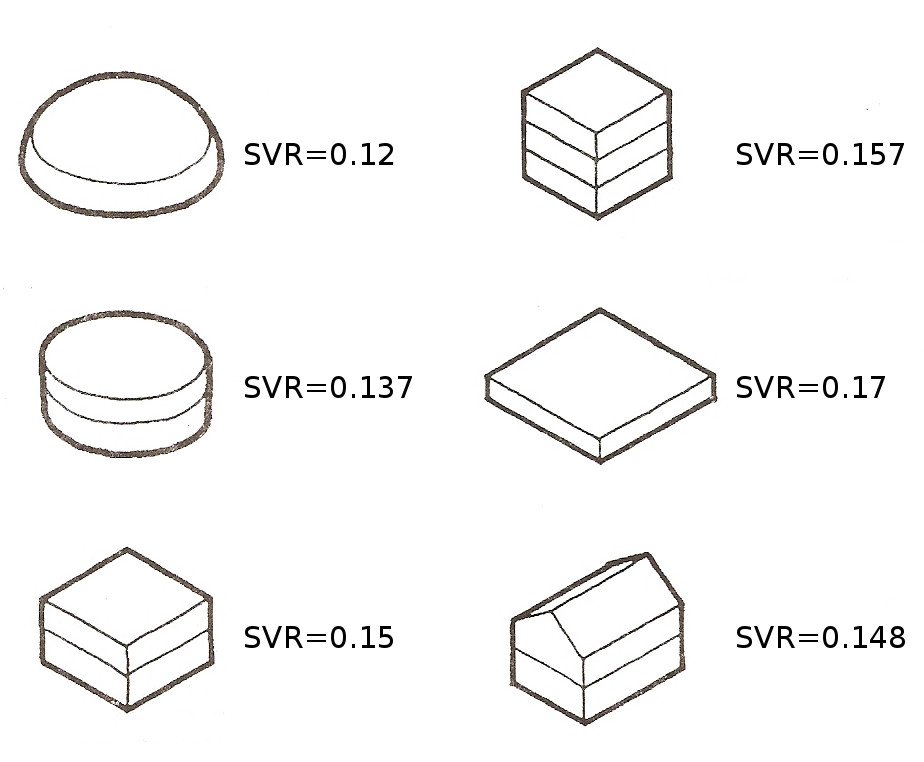
\includegraphics[width=\textwidth]{./Images/3-SVR}
			\caption{Surface-to-Volume Ratios}
			\label{fig:SVR}
		\end{figure}
	\item Compaction of Building Shape; with the same basic building shape, the SVR can be decreased using compaction, or greatly increased with		  lack of it (figure \ref{fig:Compaction}).
		\begin{figure}[H]
			\centering
			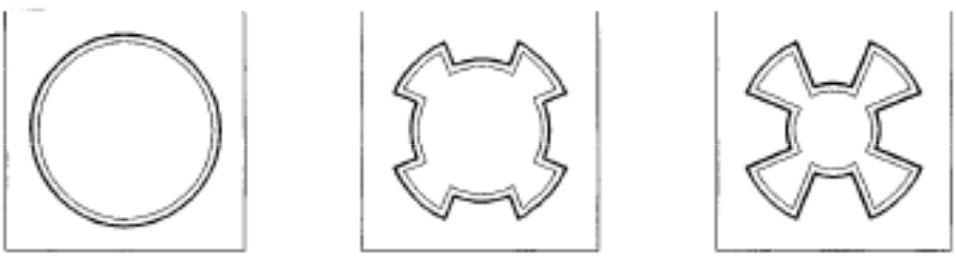
\includegraphics[width=\textwidth]{./Images/4-Compaction}
			\caption{Building Envelope Compaction}
			\label{fig:Compaction}
		\end{figure}
	\item Porosity; inner courts can create what may be called porosity of building envelope, which increases surface to volume ratio (figure 		\ref{fig:Porosity}).
		\begin{figure}[H]
			\centering
			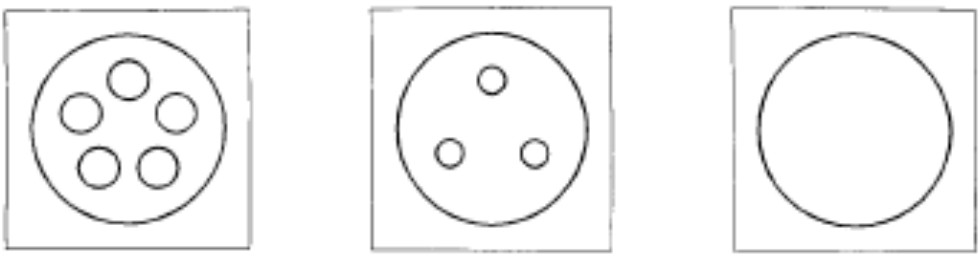
\includegraphics[width=\textwidth]{./Images/5-Porosity}
			\caption{Building Envelope Porosity}
			\label{fig:Porosity}
		\end{figure}
\end{enumerate}

\paragraph{Orientation}\mbox{}

Building orientation affects thermal performance mainly in two ways:
\begin{enumerate}
	\item The way the building perceives incident solar rays, which is dependant on the latitude of the location, and building envelope form. It should be noted that in some cases the effect of orientation is limited only to internal functions being performed in internal spaces facing a specific orientation. Buildings that are affected the most by their orientation are the ones that have big length to width ratio ---or elongated forms--- or highly non-uniform forms. (figure \ref{fig:orientation}).
		\begin{figure}[H]
			\centering
			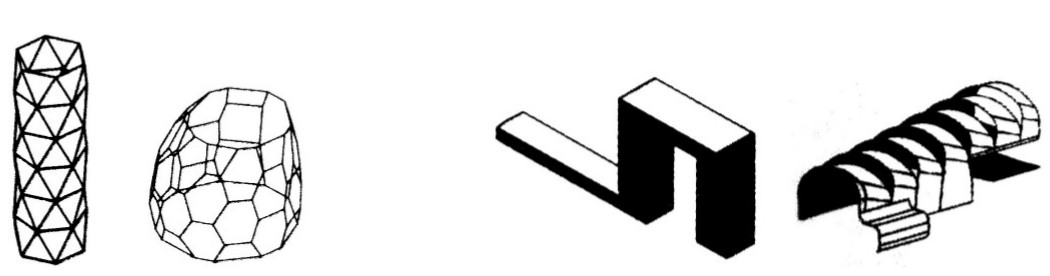
\includegraphics[width=13cm]{./Images/6-Orientation}
			\caption[Effect of Building Orientation]{In this example, the two buildings on the right would be greatly affected by their orientation in relation to the sun's position, while the two on the left are not affected except in terms of choosing internal space functions \cite{foa04}}
			\label{fig:orientation}
		\end{figure}
	\item Wind direction, which is not within the scope of this thesis.
\end{enumerate}

\paragraph{Shading}\mbox{}

What is referred to here as shading is the casting of shadow from the building onto itself; i.e. the obstruction of direct solar rays incidence on one part of the building using another.

Shading is closely related to orientation of the building, or even a direct result of it, however, it is not the only factor affecting it. The geometry of the building can greatly affect shading; an example would be part of the fa\c{c}ade which is a large cantilever hanging over lower floors (see the example in figure \ref{fig:ShadingCntlvr}).

\begin{figure}[H]
	\centering
	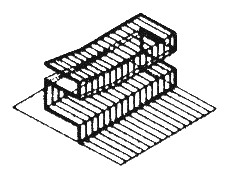
\includegraphics[width=7cm]{./Images/7-Cantilever}
	\caption[Envelope Shading]{A large part of the envelope can be facing the sun's direction but still be shaded under the cantilever parts of the building envelope \cite{foa04}}
	\label{fig:ShadingCntlvr}
\end{figure}

\paragraph{Surface Material Properties}\mbox{}

This is discussed at length in Chapter 3. Reference should be made to section \ref{sec:SolarHeatGain}, and the equation provided thereof as a basis for assigning parameters to materials such as reflectance, and to be iteratively modified through different generations of running the optimisation algorithm.

\paragraph{Fenestration Size, Shape and Position}\mbox{}

There have been several examples of the effect of opening size, shape and position on the thermal performance of a building envelope in the previous chapter, such as the Responsive Fa\c{c}ade Design System (see section \ref{sec:RFDS}) and the Generative System Method (see section \ref{sec:GSM}).

The size of fenestration is often constrained by the required amount of natural daylight for internal spaces, since both are inversely proportional. Position and shape are also important factors to be considered in the simulation.

Fenestration is almost always present in any building, however, with the exception of envelopes such as tent structures (figure \ref{fig:tent}). The absence of fenestration will render in most cases the following variables obsolete: \begin{inparaenum} \item Glazing Material, \item Closing Mechanism, and \item External Shading.\end{inparaenum}

\begin{figure}[H]
	\centering
	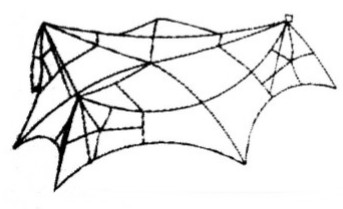
\includegraphics[width=8cm]{./Images/8-Tent}
	\caption[Tent Structure]{A tent structure as an example would not be affected by fenestration variables}
	\label{fig:tent}
\end{figure}
\paragraph{Glazing Material}\mbox{}

The same concept of surface material properties applies to glazing material; the necessity of inputting glazing material properties is that it greatly affects algorithms that specifically target openings for optimisation; in other words, if the openings are double or triple glazed, the opening size can be much larger with the same performance of a smaller opening with single clear glazing.

\paragraph{Closing Mechanisms}\mbox{}

This allows for options such as louvers to be introduced into the design to increase the thermal performance of the envelope while considerably widening the range of opening sizes above the target performance.

\paragraph{External Shading}\mbox{}

This form of shading is designed to protect internal spaces from unwanted solar rays entering through openings (i.e. fenestration). The different forms of external shading have been explained in Chapter 3 (refer to page \pageref{Shading}).

\clearpage
\subsection{Virtual Modelling and Simulation}
\label{sec:SimulationModel}

\subsubsection{Building Model}

As stated in section \ref{sec:Stage3}, the building enelope model must be parametric. The parameters and their values must be exportable to a file format recognizable by the simulation programme (\emph{e.g.} gbXML) in case the modelling is done outside the simulation programme, which will require exchange of information between two separate programmes.

\subsubsection{Simulation Programme}
Different simulation programs have been discussed relatively at length in Chapter 3 (section \ref{sec:SimulationPrograms}). The points to be considered when choosing a simulation program are as follows:

\begin{enumerate}
	\item The features and capabilities of each simulation program; the suitability of the provided list of features will depend on the kind of work being done. In case of an experiment with narrow scope and an interest in producing many results as a basis for statistical analysis (a good example being this thesis, which focuses on thermal performance of building envelopes through passive solar design), a program which is highly efficient in this particular task is preferable. This where comparative analysis studies such as the one shown earlier (see figure \ref{fig:SimProg1}, Table 2: \emph{Building Envelope, Daylight and Solar}) are very beneficial in determining which simulation programs have specific features to suite the work.

		Where the work being carried out is related to real-life projects, with interest in all aspects affecting the environmental performance of the building, it is usually the simulation program which covers most of the features shown in figures \ref{fig:SimProg1} and \ref{fig:SimProg2} is chosen.
	
	\item The ability to directly input programming code or script into the simulation programme. This was evident in Chapter 4, where the ability to use scripts and programming languages such as Lua or to input optimisation algorithms into the simulation programme is essential.
\end{enumerate}

\clearpage
\subsection{Programming and Optimisation}

The main focus of this thesis is the utilisation of algorithm in architectural design, particularly in thermal design of building envelopes; and the subject has been discussed in several parts of the thesis from different points of view.

Another aspect of most importance at this point is knowing which algorithms are most suited to the needs of the architect. As seen in the previous chapters, algorithms have different concepts; many are derived from or simulate natural evolution and growth in one way or another, others are very visual in that they detect specific shapes and transform them according to some given rule, and so on. The algorithms shown in this thesis have all been proved useful in architectural design, and specifically in thermal design.

However, having reached this point, where different building envelopes have different priorities in terms of thermal design criteria, and preferences with regards to simulation and environmental modelling programmes, it is necessary to choose the most efficient algorithm for the job. Below are some of the main points to be considered.

\subsubsection{Performative Algorithms}

Many optimisation algorithms exist other than those discussed so far, but the heuristic optimisation algorithms are usually the fastest and are fairly efficient, at least as far architectural design is concerned, and in most cases of thermal design these are the primary concerns.

Upon studying the comparative analysis of performative algorithms (refer to table \ref{tab:OptCmp}), the main elements affecting the choice of algorithm would be as follows.

\paragraph{Speed at Finding the Global Optimum}\mbox{}\vspace{-0.4cm}

As mentioned earlier in the thesis, search methods such as \emph{Brute Force}\footnote{A search method which examines \emph{all} individual solutions in a solution space (discrete values).} would theoratically have a 100\% chance of locating the global optimum; however, this comes at the price of speed. Complex problems could take days or weeks to find the global optimum since it would need to try out all possible solutions within a solution space, which could be millions or virtually infinite.

Therefore, an algorithm that can find highly elite solutions within the solution space within a short time are always preferred. Generally speaking, of the three algorithms, \emph{Simulated Annaeling} is fast enough if the solution space is not exceptionally large, and focuses on finding the single global optimum of the solution space.

\paragraph{Architectural Alternatives}\mbox{}\vspace{-0.4cm}

When a purely engineering problem is being solved using a search method, the global optimum is usually the only concern. However, when the aesthetic aspect of the solution is of concern, such as in architectural solutions, the possibility of providing alternatives in the form of elite solutions is of very high importance.

Of the three algorithms, \emph{Genetic Algorithms} is the one that satisfies this need to the greatest extent.

\paragraph{Search Efficiency in Large Solution Spaces}\mbox{}\vspace{-0.4cm}

Finding the optimum solutions is the main aim of the optimisation, and therefore, the ability to locate as many of them and as close to the global optimum as possible is a major element to be considered in the choice of algorithm. If the solution space is very large, the possibility of finding those solution will be weaker.

\emph{Tabu Search} uses a memory-based technique of search that is very efficient in analysing a large solution space, and ensures that the final solutions either contain the global optimum, or are very close to it.



\subsubsection{Generative Algorithms}

As an addtional option, if the building model had been created using a Generative Algorithm, the generating elements could be optimised instead of the architecture features. The following elements are the possible parameters to be optimised in that case:

\subparagraph{Control Constraints}

Each envelope form --- which is presumed to be at least conceptually defined to the point where it can be categorised under one of FOA envelope categories --- can be generated with different control techniques of the form evolution; this control comes in the form of constraints which are predefined by the algorithm use.

An example would be Shape Grammars; its constraints are colours, labaels and axis; while the constraints of Cellular Automata are state, neighbour and location\ldots and so on. So in order to control the evolution of the generated form, one must choose the most fitting method of control over the generating of envelope form.

The different constraints of each algorithm can be seen in table \ref{tab:GenerativeRecap}.

\subparagraph{Building Blocks and Unit Types}

The building blocks of different algorithms are the smallest units used by the algorithm; which is important since some algorithms might not be compatible with the desired forms. For example, Cellular Automata's building blocks are cells, while Shape Grammar's are basic shapes such as triangles\ldots{}etc.

It should be noted, that combinations of generative algorithms are possible, an example is shown as in figure \ref{3dCAArch}, where an algorithm similar to shape grammars is responsible for modifying the final result of cellular automata generations.

\subsubsection{Multi-criterion Optimisation}

Many of the cases presented in chapter 4 have showcased optimisation of envelopes with regard to only one variable; i.e. single-criterion optimisation (albeit with the exceptions of sections such as \ref{sec:KendallPavilion}), which was for the sake of making a clear and simple illustration of one concept or another. However, thermal optimisation in real world will almost always demand optimisation with more than one variable taken into consideration.

New problems will present themselves when shifting from single to multiple criterion optimisation, but by far the most important and influential is the problem of \emph{variable weighting system}, which is essentially the importance of each variable (external shading, fenestration\ldots etc.) in relation to the other variables. This should be studied and planned carefully by the architect, as conflicting variables will often demand very different solutions for each to be at optimum performance, and therefore the effect of each on the overall performance should be studied by the architect, possibly with the support of modelling and environmental simulation programs.

Another solution which in some cases might be practical, is to create reference points within the architectural space from which to measure the overall performance of the building envelope regardless of each variable and be used as the driving force behind the optimisation algorithm.


\clearpage
\section{Examples by Envelope Type}

At this point, the information provided so far in this chapter should be sufficient as a guide on how to design a thermally efficient building envelope using algorithm. The procedure has also been summarised for convinience in the following flowchart.

Using the flowchart, a number of examples will be presented to show the different outcomes depending on the different envelope forms.

\clearpage
\begin{sidewaysfigure}[h]
	\centering
	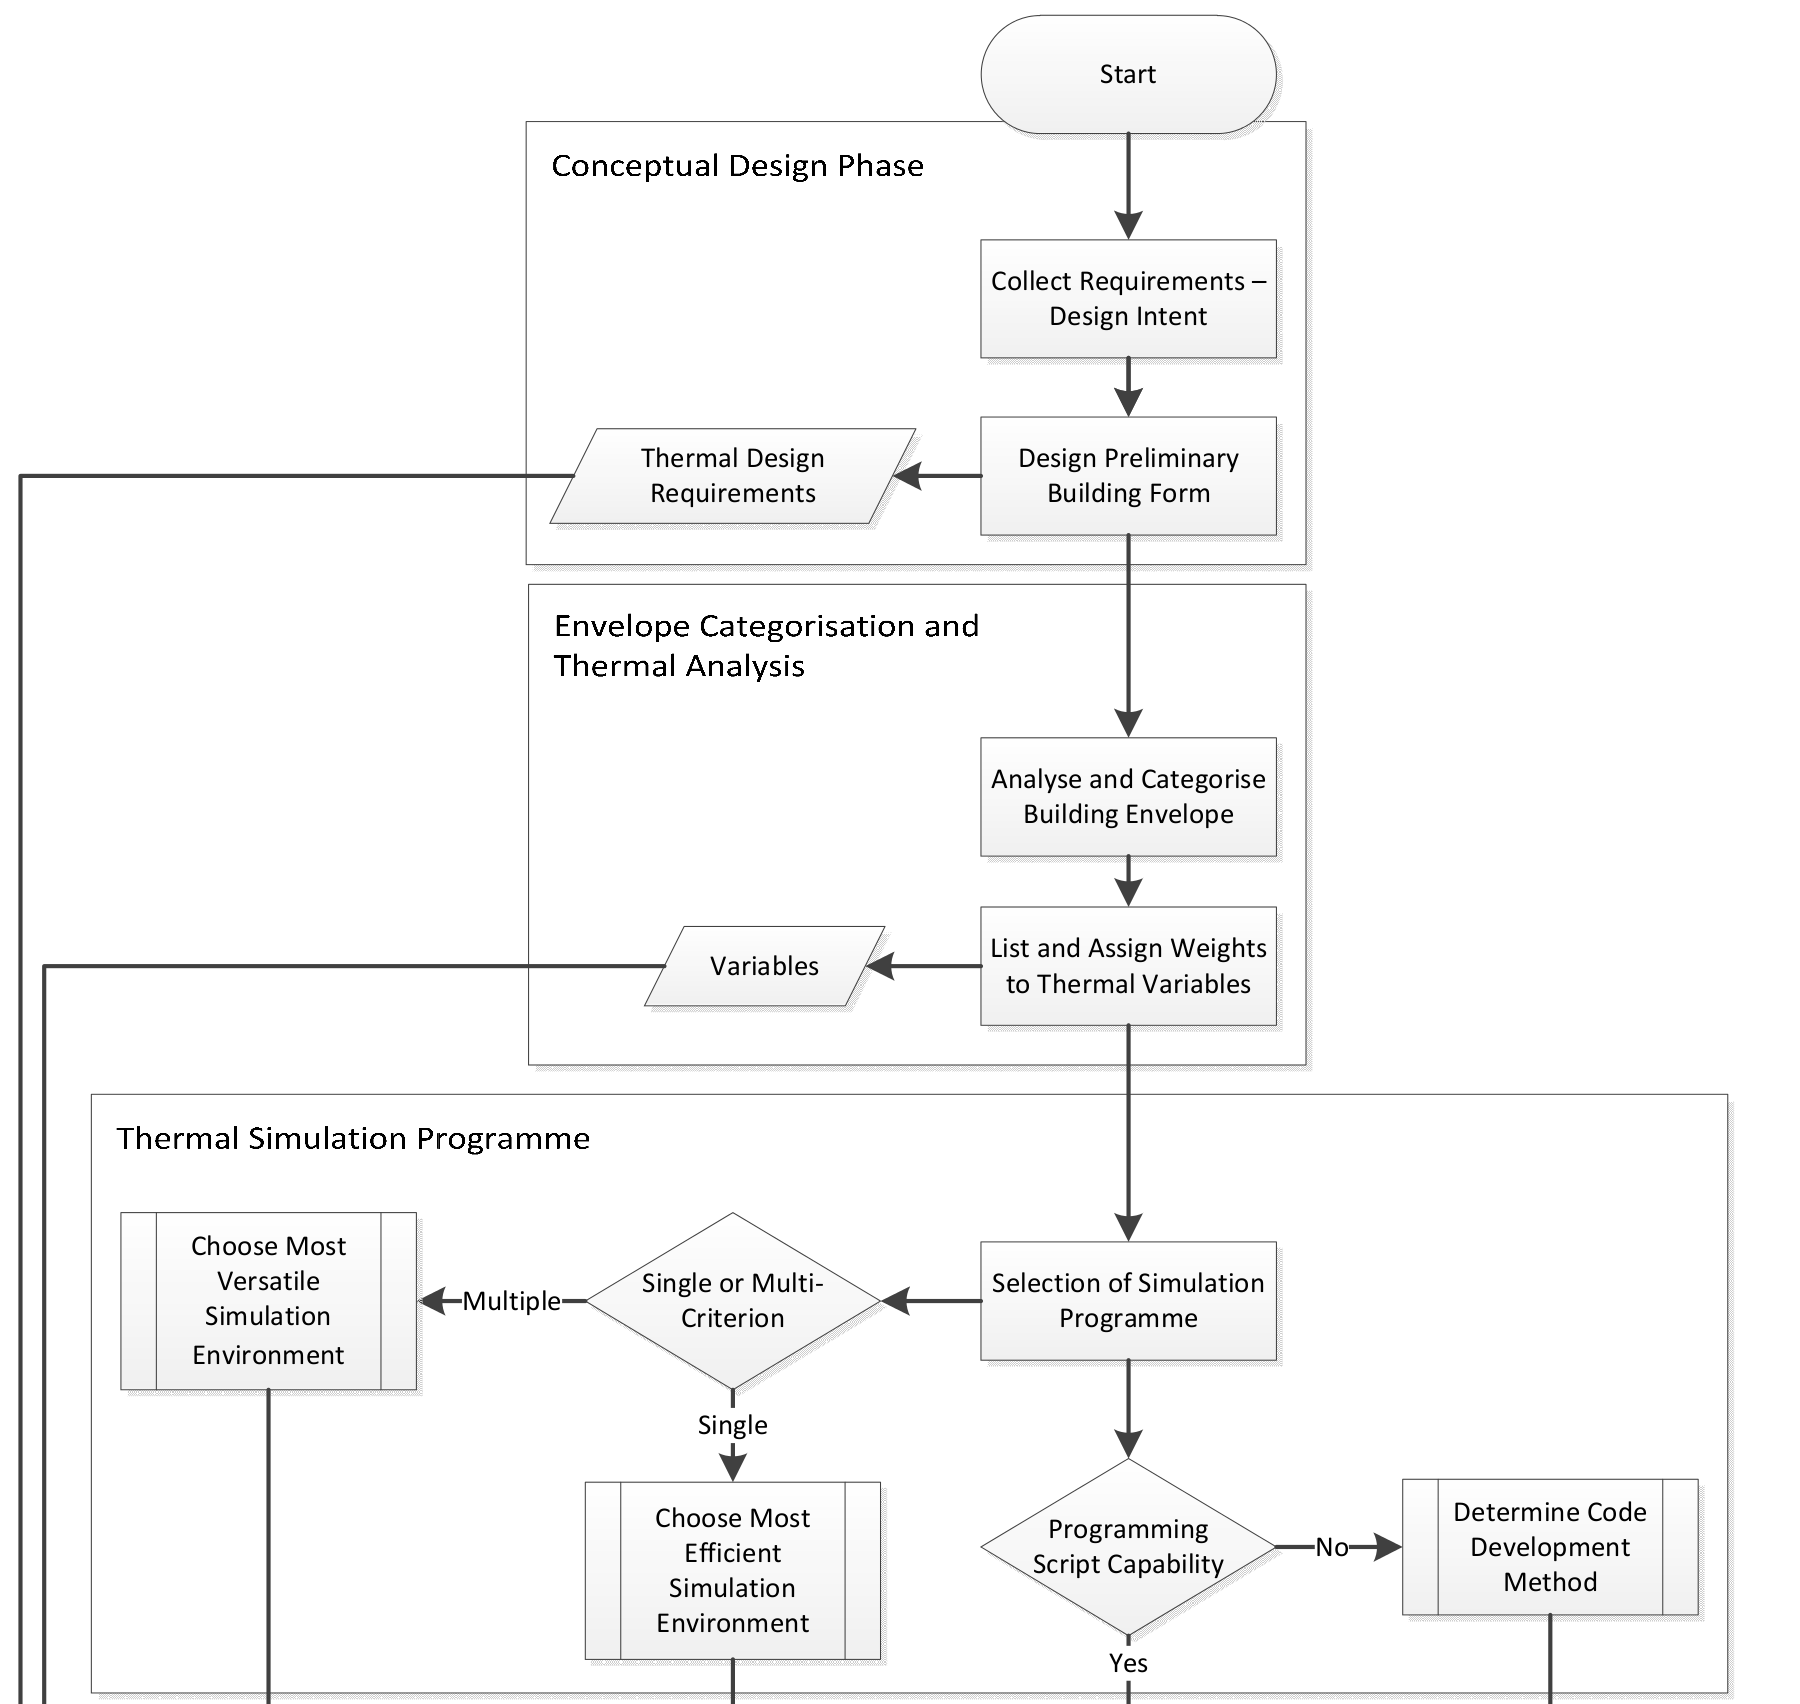
\includegraphics[width=18cm]{./Images/9a-Flowchart}
\end{sidewaysfigure}

\begin{sidewaysfigure}[h]
	\centering
	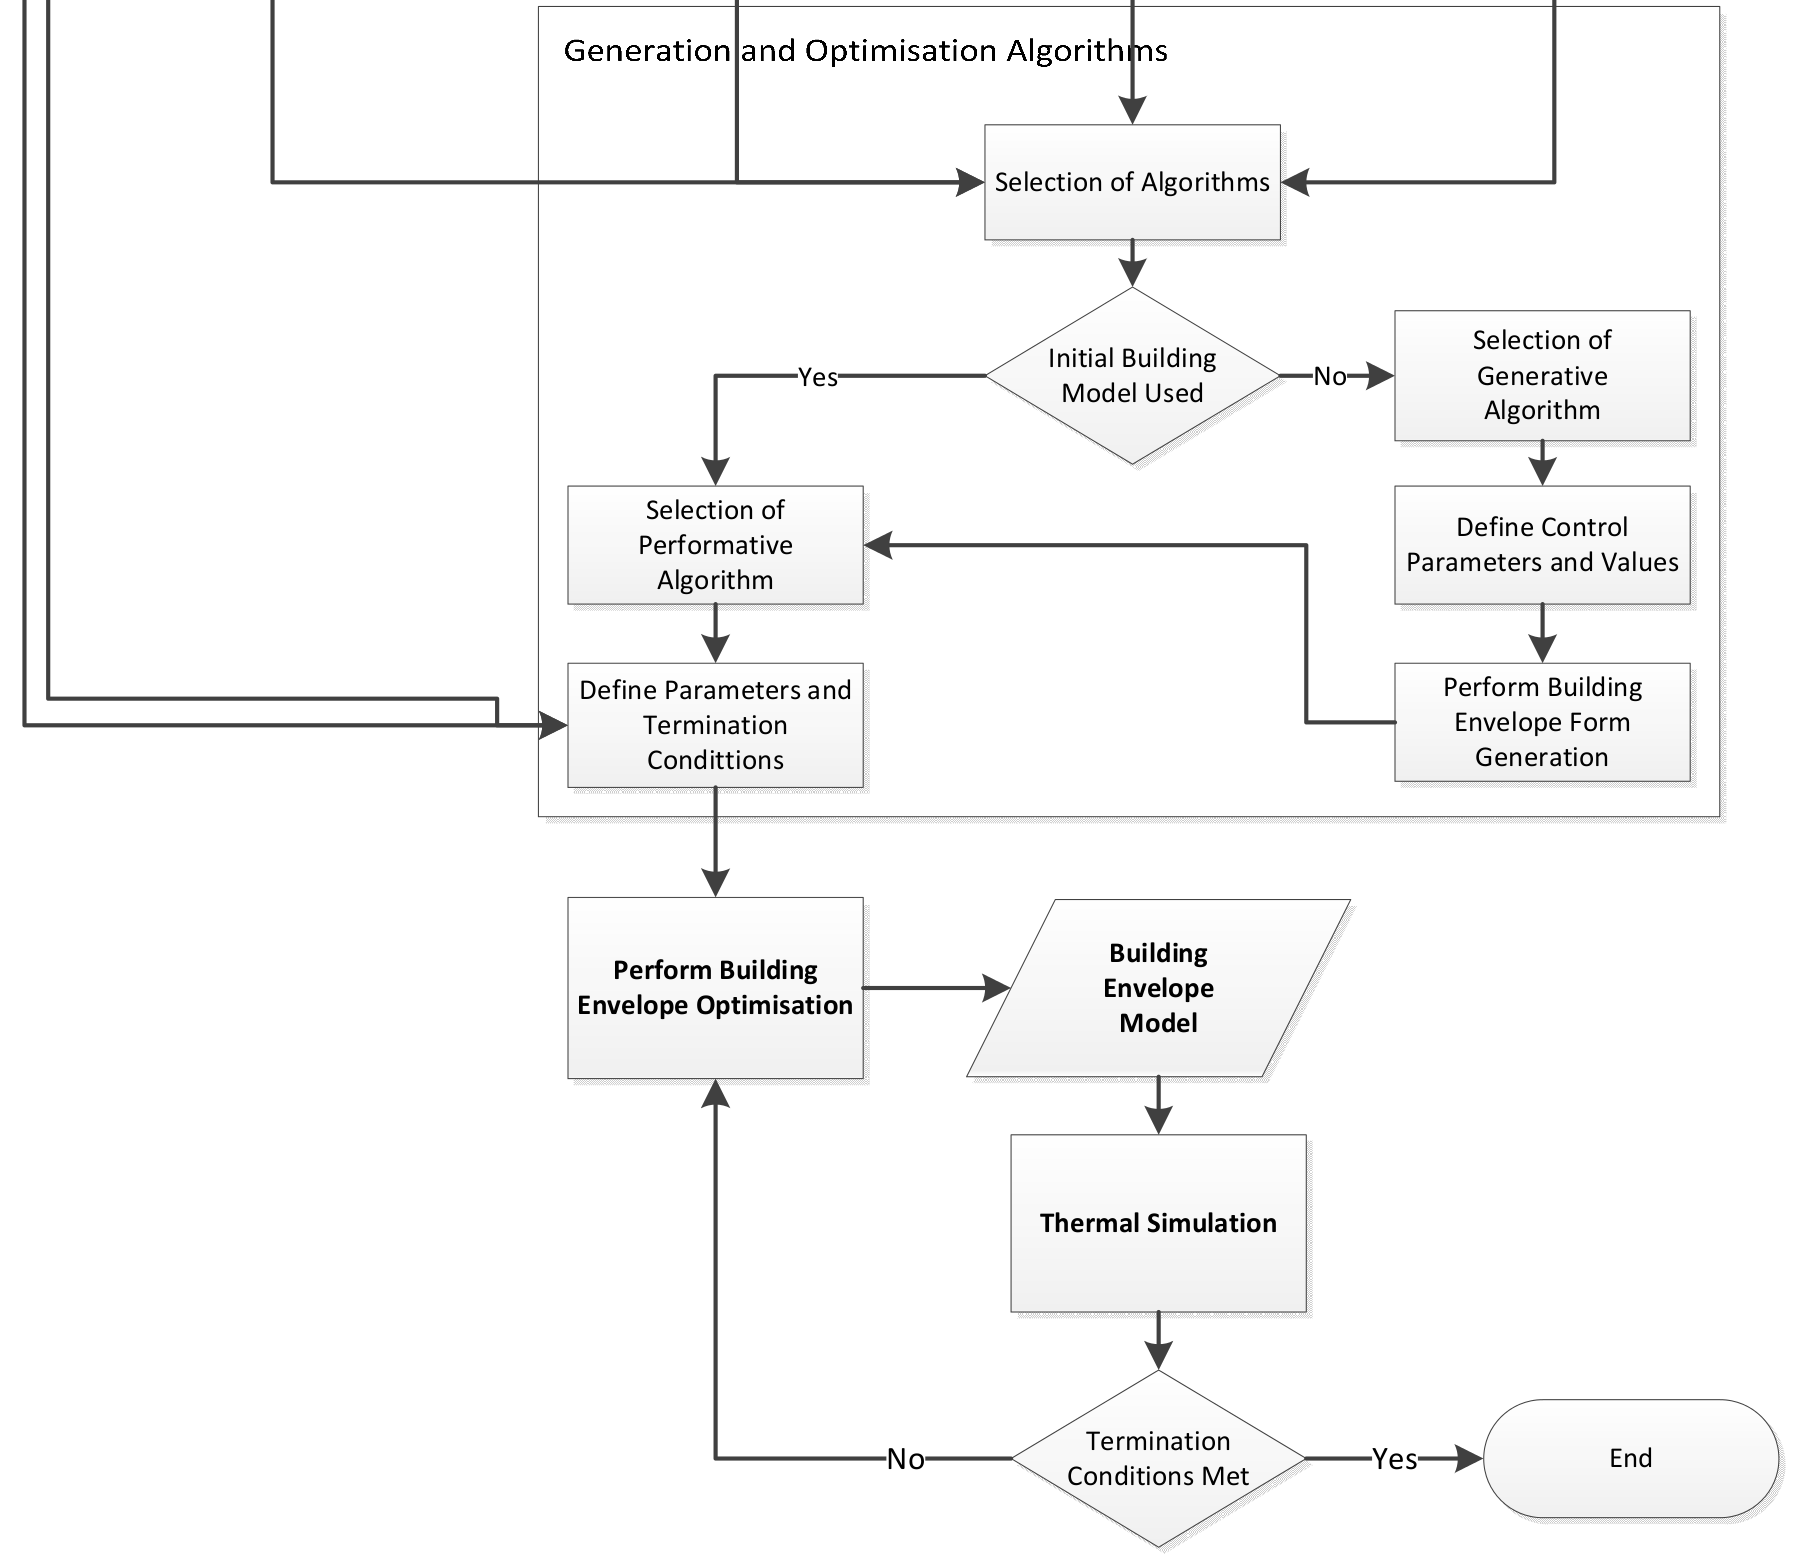
\includegraphics[width=18cm]{./Images/9b-Flowchart}
\end{sidewaysfigure}

\begin{sidewaysfigure}[h]
	\centering
	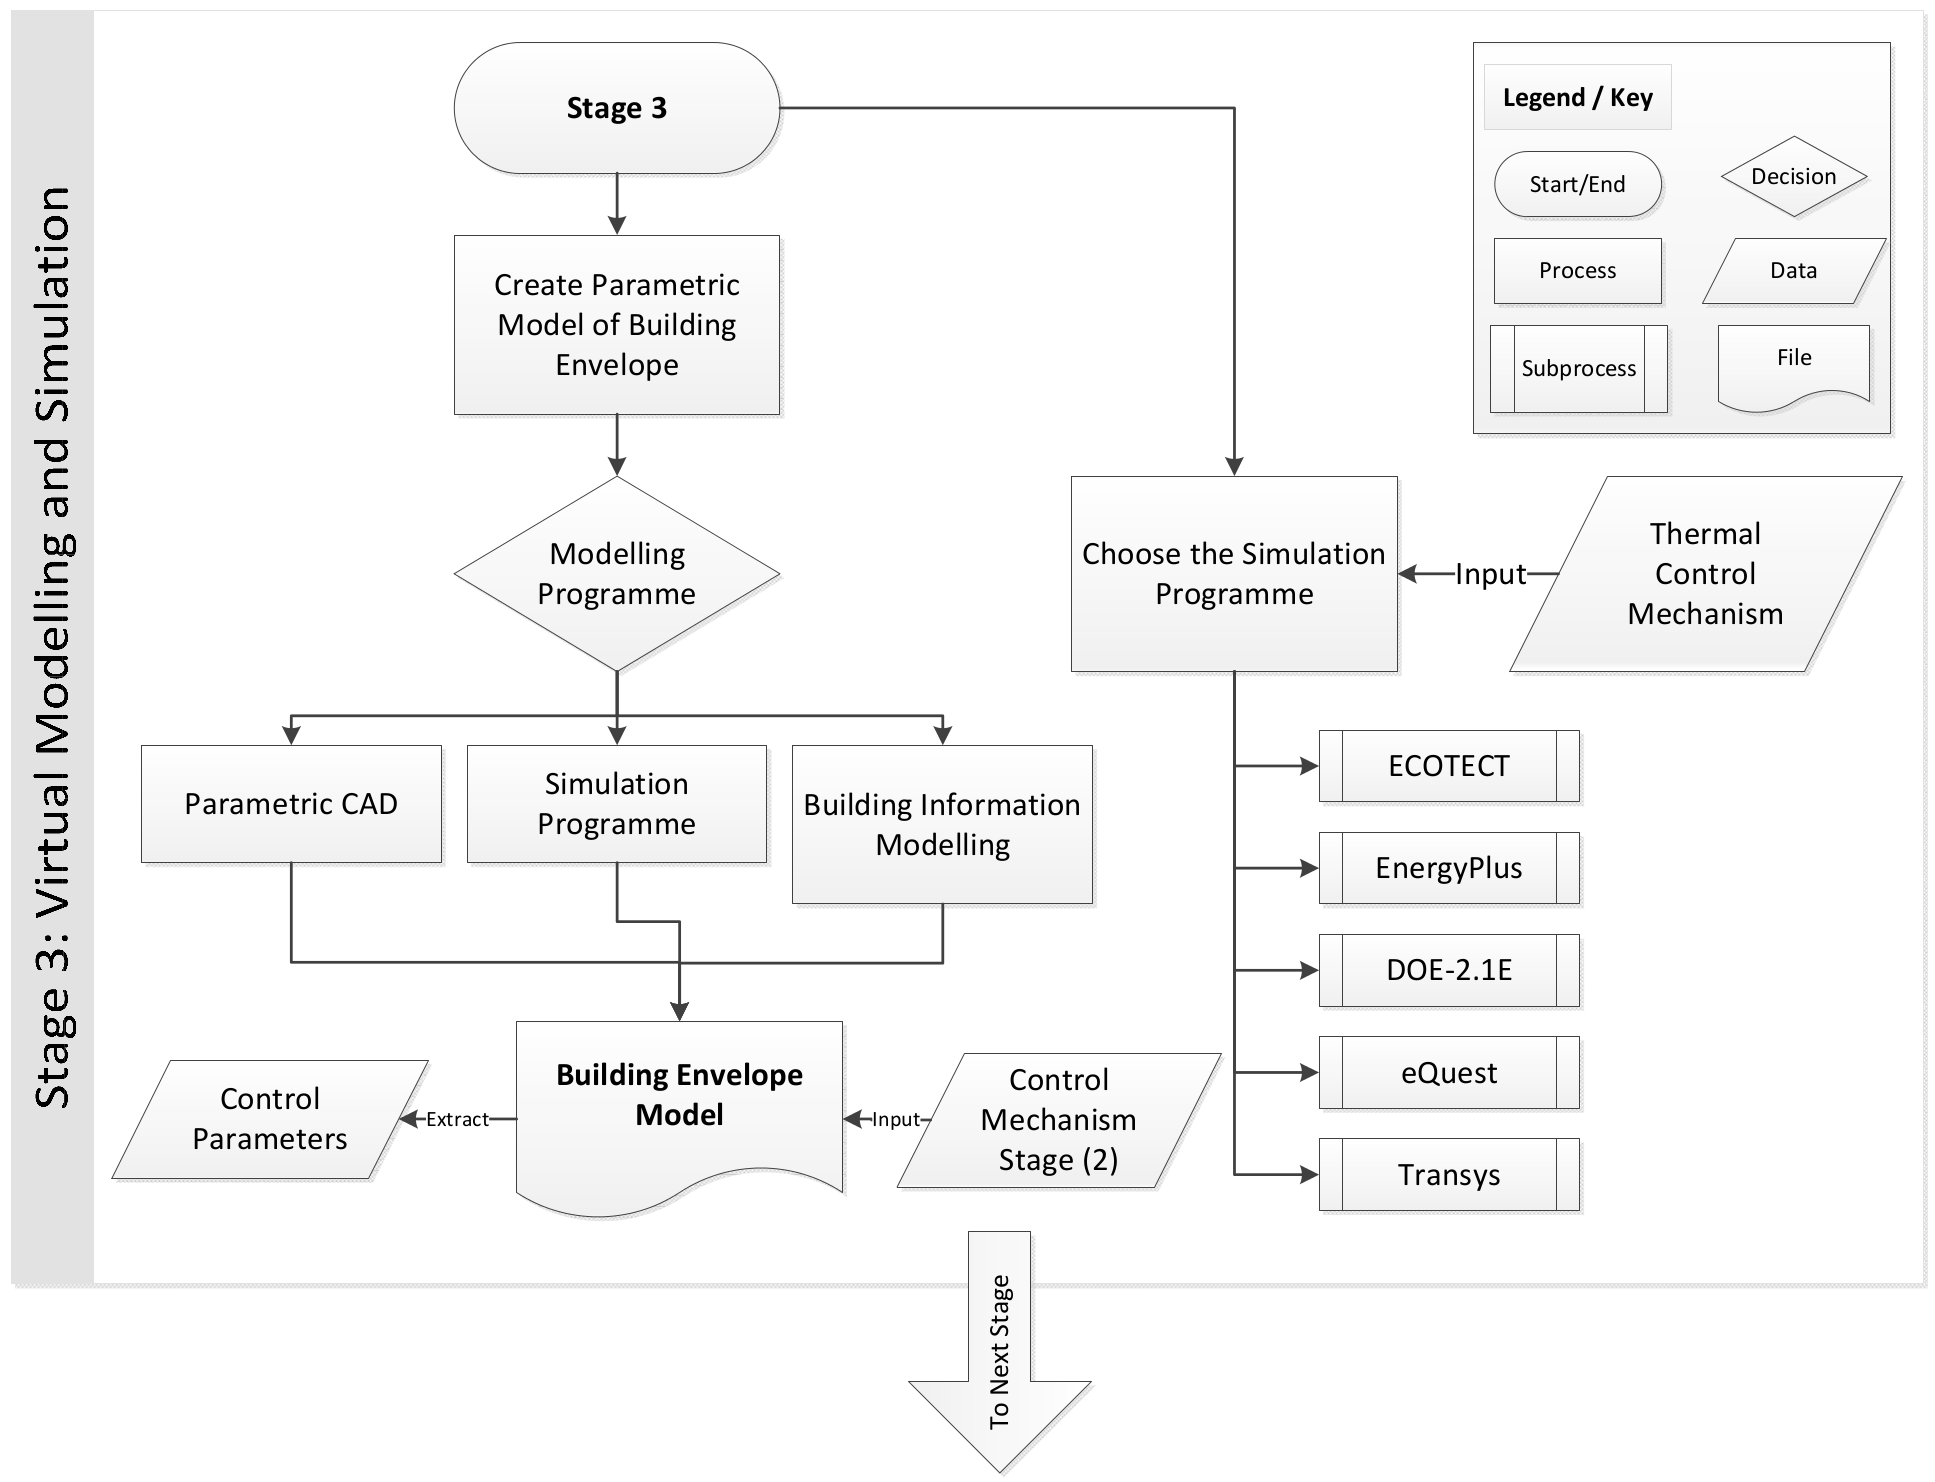
\includegraphics[width=18cm]{./Images/9c-Flowchart}
\end{sidewaysfigure}

\begin{sidewaysfigure}[h]
	\centering
	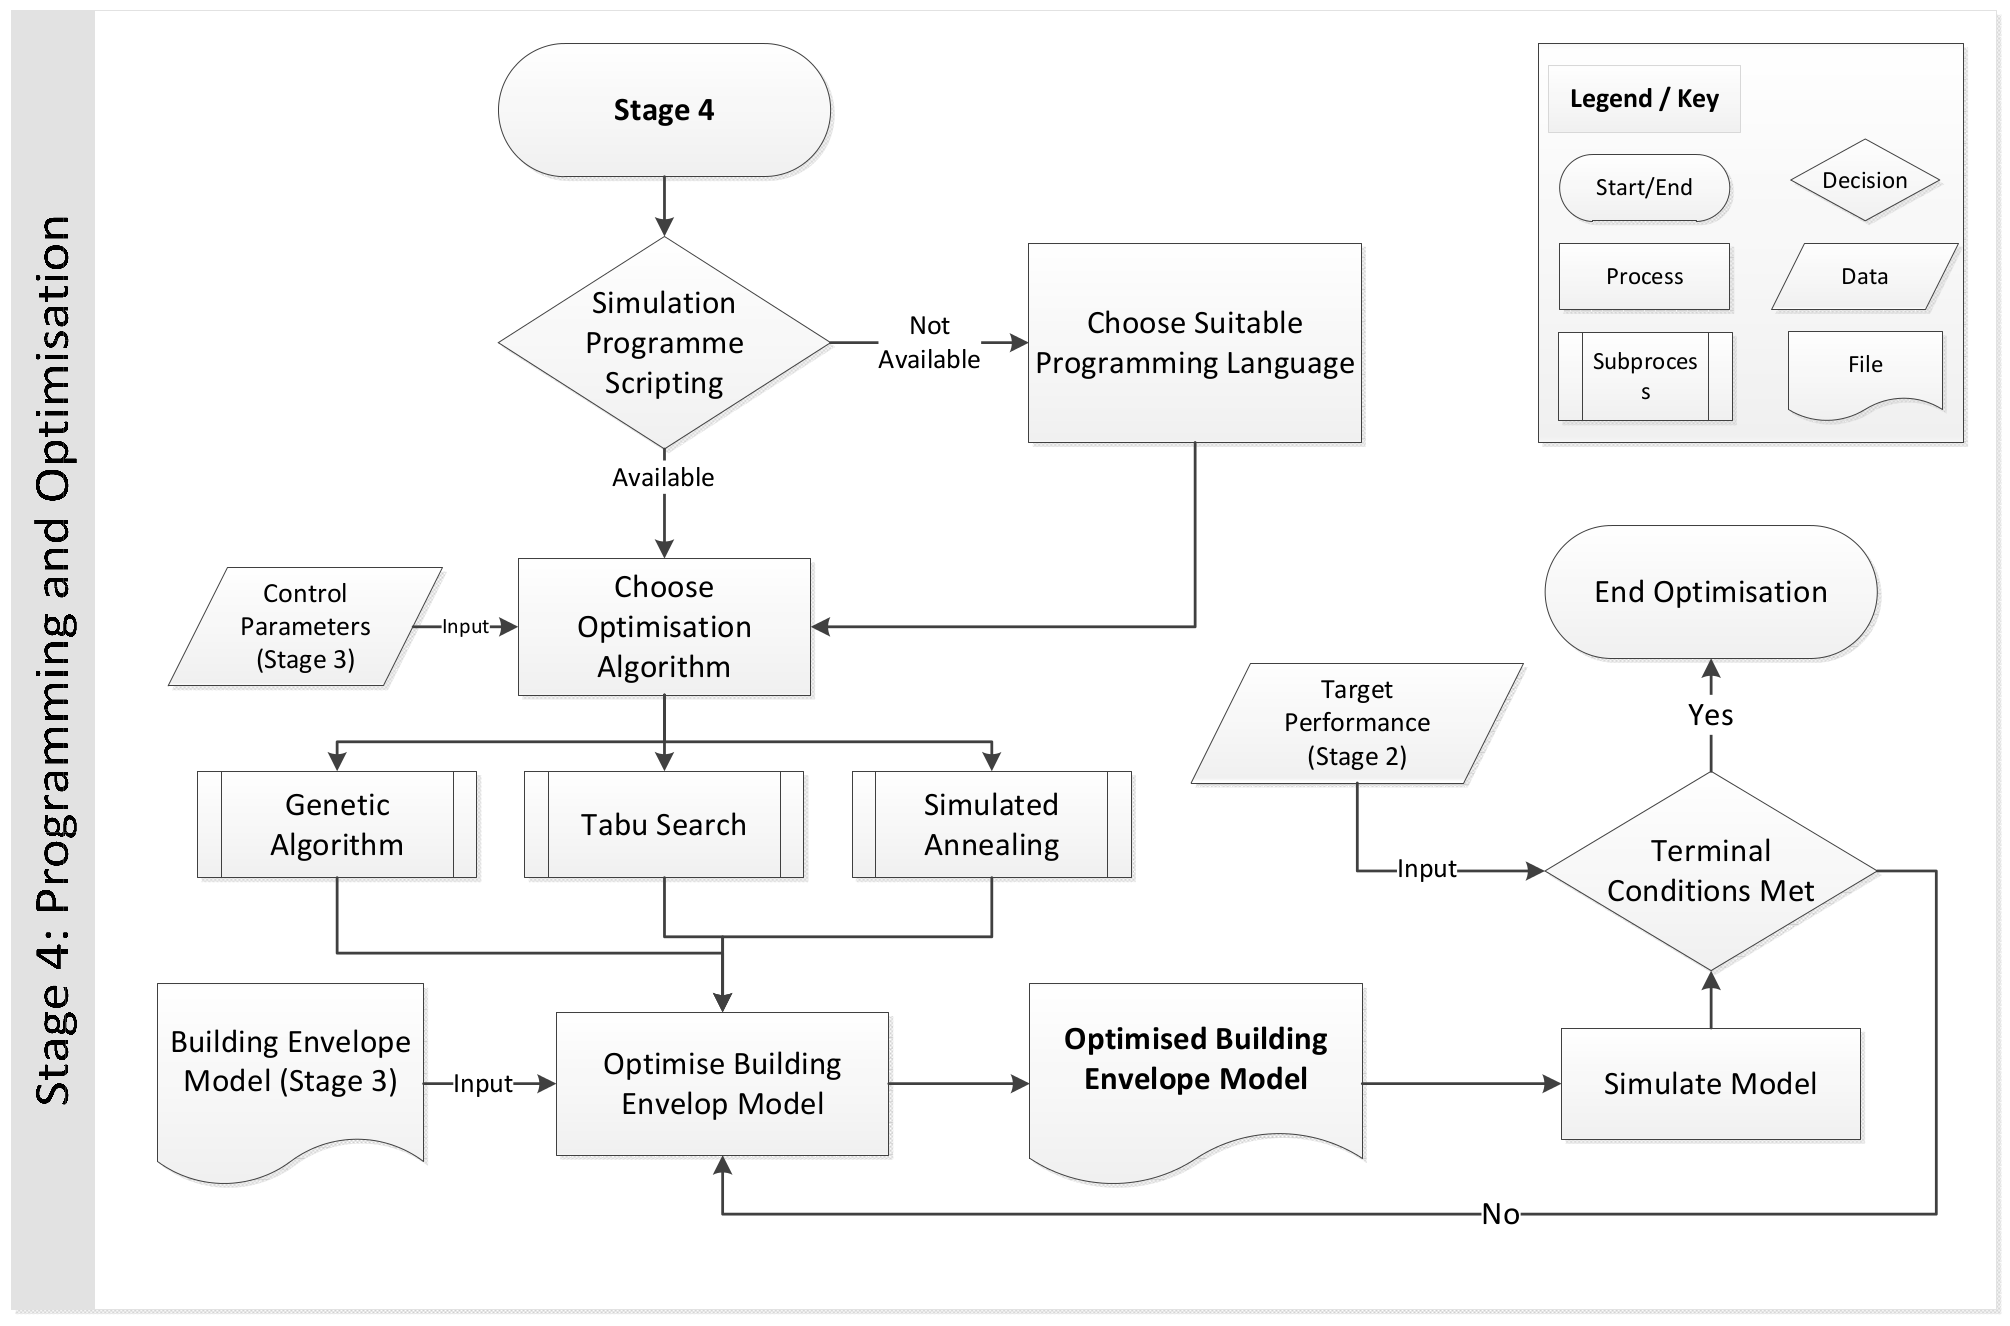
\includegraphics[width=18cm]{./Images/9d-Flowchart}
\end{sidewaysfigure}


\clearpage
\subsection{Envelope A}

\paragraph{Stage 1: Analysis of Envelope Form}\mbox{}\\[2mm]

Two main objectives are achieved in this stage; \begin{inparaenum}[a)] \item development of the bulding envelope schematic design and its categorisation, and \item determining the internal space functions.\end{inparaenum}

Assuming that at this point the Schematic Design of the building envelope had been developed; proceed to the next step of categorising the envelope.

\setlength{\columnseprule}{0pt}
\begin{multicols}{2}
	\paragraph{Building Envelope Category}\mbox{}\\
	\vspace {0.5cm}	
	\small \textsc{\textbf{Function:} Envelope\\
	\vspace {0.3cm}
	\textbf{Faciality:} Single Face\\
	\vspace {0.3cm}
	\textbf{Balance:} Constant $\rightarrow$ Parallel\\
	\vspace {0.3cm}
	\textbf{Discontinuity:} Planar\\
	\vspace {0.3cm}
	\textbf{Orientation:} Striated\\
	\vspace {0.3cm}
	\textbf{Geometry:} \emph{Not Applicable}\\
	\vspace {0.3cm}
	\textbf{Diversification:} Patterned\\}
	\normalsize
	\columnbreak
	\begin{figure}[H]
		\centering
		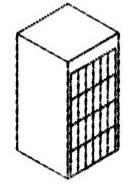
\includegraphics[width=0.35\textwidth]{./Images/10-Envelope1}
	\end{figure}
\end{multicols}
\vspace{-5mm}

The building geometry can be categrised as the fundemental or basic envelope form that corresponds to the most basic building structure. It is planar and unifrom, with no particularly significant geometrical features that could affect the thermal performance of the envelope.

Along with the schematic design and categorisation of the building envelope, the internal space functions according to project requirements should determined and documented.

\paragraph{Stage 2: Design Intent - Thermal Criteria and Target Performance}\mbox{}\\

Referring to the documented project requirements and internal space functions completed in the previous stage; the architect should assign target space temperatures in the form of reference points which would be later used by the simulation programme as loctions for measurement, and by the optimisation algorithm to determine if the terminal critieria have been met or not.

According to the building category and envelope form as described in stage 1, the envelope is very planar and unifrom with no possibilites of external shading devices or different closing mechanisms, and due to the cuboid form, the surface-to-volume ratio would not have the greatest effect if envelope proportions were changed.

Therefore, the control mechanisms which would significantly affect the internal space temperatures are:
\begin{compactenum}
	\item \textsc{Surface Material Properties}
	\item \textsc{Glazing Properties}
\end{compactenum}

\paragraph{Stage 3: Virtual Modelling and Simulation}\mbox{}\\

With the relative simplicity of the building envelope, and the possibility to effectively optimise the building envelope thermal performance through optimising surafce or glazin material properties, the parametric model is very easy to define even without a sofisticated GUI (\emph{i.e.} by defining coordinates in a text file) and can thereofore be defined directly in the simulation programme.

The control mechanism chosen (Surface Material Properties) will require the variables of the equation given in section \ref{sec:ThermalBehaviour}:\emph{Thermal Behaviour of Buildings} to be defined as the parameters to be optimised.

Given the simple geometry of the building, the GUI, modelling and  visualisation capabilities of the simmulation programme are not important. However, the most accurate energy and physics simmulator would be the best option. In this case the best simmulation programme would be:

\begin{compactenum}
	\item \textsc{Energy Plus} (A shell application can be programmed on top of \textsc{EnergyPlus} using \textsc{fortran}. Requires intermediate programming experience).
	\item \textsc{doe} (Scripting language available).
\end{compactenum}

\paragraph{Stage 4: Programming and Optimisation}\mbox{}\\

The programming method in the case of \textsc{EnergyPlus} is to create a shell application on top of it which would utilise the direct optimisation of the physical parameters of the building envelope materials.

In case of using \textsc{DOE}, the GUI can be used to model the building envelope and the scripting language would be used to define the parameters and the chosen algorithm.

Given that the problem of optimising the surface material properties would not require many alternatives but rather finding the optimum solution for the problem (minimisation of heat gain), hence, the best algorithm for this problem would be:

\begin{compactenum}
\item \textsc{Simmulated Annealing}
\end{compactenum}

The model is then simmulated and the paramters are optimised iteratively until either \begin{inparaenum}[a)]\item the global optimum/minimum is found, or \item the terminal conditions are met\end{inparaenum}.

\clearpage
\subsection{Envelope B}

\paragraph{Stage 1: Analysis of Envelope Form}\mbox{}\\[2mm]

Two main objectives are achieved in this stage; \begin{inparaenum}[a)] \item development of the bulding envelope schematic design and its categorisation, and \item determining the internal space functions.\end{inparaenum}

Assuming that at this point the Schematic Design of the building envelope had been developed; proceed to the next step of categorising the envelope.

\setlength{\columnseprule}{0pt}
\begin{multicols}{2}
	\paragraph{Building Envelope Category}\mbox{}\\
	\vspace {0.5cm}	
	\small \textsc{\textbf{Function:} Envelope\\
	\vspace {0.3cm}
	\textbf{Faciality:} Single Face\\
	\vspace {0.3cm}
	\textbf{Balance:} Shifting\\
	\vspace {0.3cm}
	\textbf{Discontinuity:} Perforated\\
	\vspace {0.3cm}
	\textbf{Orientation:} \emph{Not Applicable}\\
	\vspace {0.3cm}
	\textbf{Geometry:} \emph{Not Applicable}\\
	\vspace {0.3cm}
	\textbf{Diversification:} \emph{Not Applicable}\\}
	\normalsize
	\columnbreak
	\vspace{4cm}
	\begin{figure}[H]
		\centering
		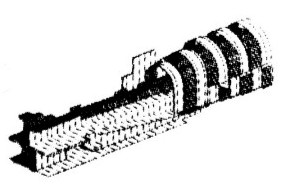
\includegraphics[width=0.5\textwidth]{./Images/13-Envelope4}
	\end{figure}
\end{multicols}
\vspace{-5mm}

This envelope form represents a fairly complex shape, with uniaxial symmetry, possibility of several material selections, shading devices and is significantly affected by building orientation. However, the building envelope is a mixture of planar and shifting surfaces (such as the vault structure), which can give mixed results on change of orientation.

Along with the schematic design and categorisation of the building envelope, the internal space functions according to project requirements should determined and documented.

\paragraph{Stage 2: Design Intent - Thermal Criteria and Target Performance}\mbox{}\\

Referring to the documented project requirements and internal space functions completed in the previous stage; the architect should assign target space temperatures in the form of reference points which would be later used by the simulation programme as loctions for measurement, and by the optimisation algorithm to determine if the terminal critieria have been met or not.

According to the building category and envelope form as described in stage 1, the envelope has many potential effective thermal control mechanisms, including orientation of building, shading, external shading, and possibly glazing material.

However, the control mechanisms which would significantly affect the internal space temperatures the most are:
\begin{compactenum}
	\item \textsc{Orientation}
	\item \textsc{External Shading}
\end{compactenum}

\paragraph{Stage 3: Virtual Modelling and Simulation}\mbox{}\\

The building envelope can be considered conventional and has simple geometry. However, it would be much easier to model the envelope in a GUI capable and user friendly programme. In this case, the simulation programme \textsc{ecotect} would serve as a very good choice, with the advantage of having a scripting language (\textsc{Lua}) that can facilitate programming the optimisation algorithm directly into the modeling and simulation programme.

The environmental simulation of \textsc{ecotect} is very intuitive, interactive and overall user friendly; it includes a module for simulating the sun's position at any given date and time according to the predefined latitude and longitude of the building site. This will serve as a basis for the analysis of amount of incident solar rays using different building orientation configurations.

The optimisation problem can be of multi-criterion, since the optimised paramters are fairly simple, where after the orientation is chosen, external shading configuration can be decided.

\paragraph{Stage 4: Programming and Optimisation}\mbox{}\\

The scripting language is capable of handling the internal programming of the optimisation algorithm into the simulation programme.

Optimisation of building orientation and external shading do not require heavy calculations or memory based optimisation, but the external shading configuration can benefit from the possibility of having several architectural solutions. The most suitable optimisation algorithm in this case would be 

\begin{compactenum}
\item \textsc{Genetic Algorithm}
\end{compactenum}

The model is then simmulated and the paramters are optimised iteratively until either \begin{inparaenum}[a)]\item the global optimum/minimum is found, or \item the terminal conditions are met\end{inparaenum}.

\clearpage
\subsection{Envelope C}

\paragraph{Stage 1: Analysis of Envelope Form}\mbox{}\\[2mm]

Two main objectives are achieved in this stage; \begin{inparaenum}[a)] \item development of the bulding envelope schematic design and its categorisation, and \item determining the internal space functions.\end{inparaenum}

Assuming that at this point the Schematic Design of the building envelope had been developed; proceed to the next step of categorising the envelope.

\setlength{\columnseprule}{0pt}
\begin{multicols}{2}
	\paragraph{Building Envelope Category}\mbox{}\\
	\vspace {0.5cm}	
	\small \textsc{\textbf{Function:} Envelope\\
	\vspace {0.3cm}
	\textbf{Faciality:} Single Face\\
	\vspace {0.3cm}
	\textbf{Balance:} Constant $\rightarrow$ Parallel\\
	\vspace {0.3cm}
	\textbf{Discontinuity:} Planar\\
	\vspace {0.3cm}
	\textbf{Orientation:} Oriented\\
	\vspace {0.3cm}
	\textbf{Geometry:} Discontinuous\\
	\vspace {0.3cm}
	\textbf{Diversification:} \emph{Not Applicable}\\}
	\normalsize
	\columnbreak
	\vspace{3.5cm}
	\begin{figure}[H]
		\centering
		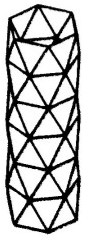
\includegraphics[width=0.18\textwidth]{./Images/18-Envelope9}
	\end{figure}
\end{multicols}
\vspace{-5mm}

This envelope form represents the typical high rise towers of the late 20\textsuperscript{th} century, which lacks any shading devices and rarely has controllable fenestration. This envelope's thermal performance depends mainly on the curtain wall materials.

Along with the schematic design and categorisation of the building envelope, the internal space functions according to project requirements should determined and documented.

\paragraph{Stage 2: Design Intent - Thermal Criteria and Target Performance}\mbox{}\\

Referring to the documented project requirements and internal space functions completed in the previous stage; the architect should assign target space temperatures in the form of reference points which would be later used by the simulation programme as loctions for measurement, and by the optimisation algorithm to determine if the terminal critieria have been met or not.

According to the building category and envelope form as described in stage 1, and assuming that as with most similar high rise buildings that prominent material of the shell would be Glazing, then the most effective control mechanism is: 

\begin{compactenum}
	\item \textsc{Glazing Material}
\end{compactenum}

\paragraph{Stage 3: Virtual Modelling and Simulation}\mbox{}\\

The modelling programme is of no particular significance, therefore, a parametric CAD programme would be sufficient. The simmulation programme which is most capable and efficient in the calculation and simulation of building envelope heat gain is \textsc{EnergyPlus}.

\paragraph{Stage 4: Programming and Optimisation}\mbox{}\\

The calculation of heat gain of multi-layered transparent elements can be consuming of processing and calculation power if done with acceptable precision, therefore it is a fairly complex problem. The most efficient search algorithm for this case would be:

\begin{compactenum}
\item \textsc{Tabu Search}
\end{compactenum}

The model is then simmulated and the paramters are optimised iteratively until either \begin{inparaenum}[a)]\item the global optimum/minimum is found, or \item the terminal conditions are met\end{inparaenum}.


\clearpage
\subsection{Envelope D}

\paragraph{Stage 1: Analysis of Envelope Form}\mbox{}\\[2mm]

Two main objectives are achieved in this stage; \begin{inparaenum}[a)] \item development of the bulding envelope schematic design and its categorisation, and \item determining the internal space functions.\end{inparaenum}

Assuming that at this point the Schematic Design of the building envelope had been developed; proceed to the next step of categorising the envelope.

\setlength{\columnseprule}{0pt}
\begin{multicols}{2}
	\paragraph{Building Envelope Category}\mbox{}\\
	\vspace {0.5cm}	
	\small \textsc{\textbf{Function:} Envelope\\
	\vspace {0.3cm}
	\textbf{Faciality:} Single Face\\
	\vspace {0.3cm}
	\textbf{Balance:} Constant $\rightarrow$ Parallel\\
	\vspace {0.3cm}
	\textbf{Discontinuity:} Planar\\
	\vspace {0.3cm}
	\textbf{Orientation:} Oriented\\
	\vspace {0.3cm}
	\textbf{Geometry:} \emph{Not Applicable}\\
	\vspace {0.3cm}
	\textbf{Diversification:} Contingent\\}
	\normalsize
	\columnbreak
	\vspace{3.5cm}
	\begin{figure}[H]
		\centering
		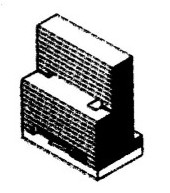
\includegraphics[width=0.4\textwidth]{./Images/11-Envelope2}
	\end{figure}
\end{multicols}
\vspace{-5mm}

This envelope form represents a typical multi-story building with modular fenestration, mid-height roofs, and is of oblong proportions.

Along with the schematic design and categorisation of the building envelope, the internal space functions according to project requirements should determined and documented.

\paragraph{Stage 2: Design Intent - Thermal Criteria and Target Performance}\mbox{}\\

Referring to the documented project requirements and internal space functions completed in the previous stage; the architect should assign target space temperatures in the form of reference points which would be later used by the simulation programme as loctions for measurement, and by the optimisation algorithm to determine if the terminal critieria have been met or not.

According to the building category and envelope form as described in stage 1, the envelope has high potential of developing external shading devices for the modular and continuous fenestration. With the proporions of the buidling and the opennings configuration, the most suitable control mechanism is:

\begin{compactenum}
	\item \textsc{External Shading}
\end{compactenum}

\paragraph{Stage 3: Virtual Modelling and Simulation}\mbox{}\\

The intuitive and graphical interface of \textsc{ecotect} is the best modelling and simulation interface for the optimisation of external shading devices. The programme also has built-in algorithms that calculate the optimum shape and size of external shading devices.

\paragraph{Stage 4: Programming and Optimisation}\mbox{}\\

Given the relative simplicity of the problem, while having direct impact on the aesthetics of the building, the most suitable search algorithm is the one that provides several alternatives for the from, which is:

\begin{compactenum}
\item \textsc{Genetic Algorithm}
\end{compactenum}

The model is then simmulated and the paramters are optimised iteratively until either \begin{inparaenum}[a)]\item the global optimum/minimum is found, or \item the terminal conditions are met\end{inparaenum}.


\clearpage	
\subsection{Envelope E}

\paragraph{Stage 1: Analysis of Envelope Form}\mbox{}\\[2mm]

Two main objectives are achieved in this stage; \begin{inparaenum}[a)] \item development of the bulding envelope schematic design and its categorisation, and \item determining the internal space functions.\end{inparaenum}

Assuming that at this point the Schematic Design of the building envelope had been developed; proceed to the next step of categorising the envelope.

\setlength{\columnseprule}{0pt}
\begin{multicols}{2}
	\paragraph{Building Envelope Category}\mbox{}\\
	\vspace {0.5cm}	
	\small \textsc{\textbf{Function:} Envelope\\
	\vspace {0.3cm}
	\textbf{Faciality:} Single Face\\
	\vspace {0.3cm}
	\textbf{Balance:} Constant $\rightarrow$ Perpindicular\\
	\vspace {0.3cm}
	\textbf{Discontinuity:} Planar\\
	\vspace {0.3cm}
	\textbf{Orientation:} \emph{Not Applicable}\\
	\vspace {0.3cm}
	\textbf{Geometry:} Continuous\\
	\vspace {0.3cm}
	\textbf{Diversification:} \emph{Not Applicable}\\}
	\normalsize
	\columnbreak
	\vspace{5.5cm}
	\begin{figure}[H]
		\centering
		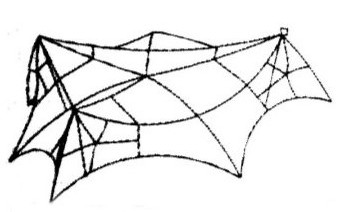
\includegraphics[width=0.5\textwidth]{./Images/22-Envelope13}
	\end{figure}
\end{multicols}
\vspace{-5mm}

This is the typical tent structure envelope form. The envelope has no opennings, it has one dominent suface material, and its thermal conductivity is usually irrelevant as the heat does not transfer by convection within the large internal spaces.

Along with the schematic design and categorisation of the building envelope, the internal space functions according to project requirements should determined and documented.

\paragraph{Stage 2: Design Intent - Thermal Criteria and Target Performance}\mbox{}\\

Referring to the documented project requirements and internal space functions completed in the previous stage; the architect should assign target space temperatures in the form of reference points which would be later used by the simulation programme as loctions for measurement, and by the optimisation algorithm to determine if the terminal critieria have been met or not.

According to the building category and envelope form as described in stage 1, the envelope does not depend on fenestration for thermal control, it is not affected by orientation, with no effective method of control self shading or creating effective external shading devices, and the surface material properties are not relevant. The only remaining control mechanism which could be of great significiance is: 

\begin{compactenum}
	\item \textsc{Surface-to-Volume Ratio}
\end{compactenum}

\paragraph{Stage 3: Virtual Modelling and Simulation}\mbox{}\\

The envelope form is complex and requires high-end nurbs modelling capabilities. therefore, the use of parametric modeling cad or building information modelling software would be needed. bim is usually preferred due to its ability to export data to gbxml format which can later on be exported to programmes such as \textsc{ecotect}.

The recommended simulation programme in this case is \textsc{ecotect}, which can receive the gbxml data from the bim model, and has a capable scripting language based on \textsc{lua}.

\paragraph{Stage 4: Programming and Optimisation}\mbox{}\\

The scripting language is capable of handling the internal programming of the optimisation algorithm into the simulation programme.

Optimisation of Surface-to-Volume Ratio will have direct and easily noticable impact on building form; therefore, the use of an algorithm which allows for alternatives is preferred:

\begin{compactenum}
\item \textsc{Genetic Algorithm}
\end{compactenum}

The model is then simmulated and the paramters are optimised iteratively until either \begin{inparaenum}[a)]\item the global optimum/minimum is found, or \item the terminal conditions are met\end{inparaenum}.


\clearpage
\subsection{Envelope F}

\paragraph{Stage 1: Analysis of Envelope Form}\mbox{}\\[2mm]

Two main objectives are achieved in this stage; \begin{inparaenum}[a)] \item development of the bulding envelope schematic design and its categorisation, and \item determining the internal space functions.\end{inparaenum}

Assuming that at this point the Schematic Design of the building envelope had been developed; proceed to the next step of categorising the envelope.

\setlength{\columnseprule}{0pt}
\begin{multicols}{2}
	\paragraph{Building Envelope Category}\mbox{}\\
	\vspace {0.5cm}	
	\small \textsc{\textbf{Function:} Envelope\\
	\vspace {0.3cm}
	\textbf{Faciality:} Single Face\\
	\vspace {0.3cm}
	\textbf{Balance:} Parallel\\
	\vspace {0.3cm}
	\textbf{Discontinuity:} Planar\\
	\vspace {0.3cm}
	\textbf{Orientation:} Non-Oriented\\
	\vspace {0.3cm}
	\textbf{Geometry:} \emph{Not Applicable}\\
	\vspace {0.3cm}
	\textbf{Diversification:} \emph{Not Applicable}\\}
	\normalsize
	\columnbreak
	\vspace{3.5cm}
	\begin{figure}[H]
		\centering
		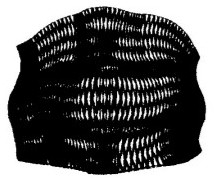
\includegraphics[width=0.5\textwidth]{./Images/21-Envelope12}
	\end{figure}
\end{multicols}
\vspace{-5mm}

This envelope form represents building that have organic, curveous form, with continuous surfaces. The architectural style is sometimes referred to as \emph{Blob Architecture}.

Along with the schematic design and categorisation of the building envelope, the internal space functions according to project requirements should determined and documented.

\paragraph{Stage 2: Design Intent - Thermal Criteria and Target Performance}\mbox{}\\

Referring to the documented project requirements and internal space functions completed in the previous stage; the architect should assign target space temperatures in the form of reference points which would be later used by the simulation programme as loctions for measurement, and by the optimisation algorithm to determine if the terminal critieria have been met or not.

According to the building category and envelope form as described in stage 1, the envelope does not respond to fenestration control mechanisms, and is highly influenced by the surface material properties, with possibility of control through Surface-to-Volume ratio of the envelope.

The most effective control mechanisms are:

\begin{compactenum}
	\item \textsc{Surface Material Properties}
	\item \textsc{Surface-to-Volume Ratio}
\end{compactenum}

\paragraph{Stage 3: Virtual Modelling and Simulation}\mbox{}\\

The envelope form is complex and requires high-end nurbs modelling capabilities. therefore, the use of parametric modeling cad or building information modelling software would be needed. bim is usually preferred due to its ability to export data to gbxml format which can later on be exported to programmes such as \textsc{ecotect}.

Although \textsc{ecotect} can receive the gbxml data from the BIM model, the calculation could need the precision of EnergyPlus instead.

\paragraph{Stage 4: Programming and Optimisation}\mbox{}\\

The scripting language is capable of handling the internal programming of the optimisation algorithm into the simulation programme.

The optimisational search problems requires heavy calculations of the effect of surface material on thermal gain considering the irregular shape and possibilities of the building reflecting on itself. The most efficient search algorithm would be:

\begin{compactenum}
\item \textsc{Tabu Search}
\end{compactenum}

The model is then simmulated and the paramters are optimised iteratively until either \begin{inparaenum}[a)]\item the global optimum/minimum is found, or \item the terminal conditions are met\end{inparaenum}.


\begin{sidewaysfigure}[htbp]
	\centering
	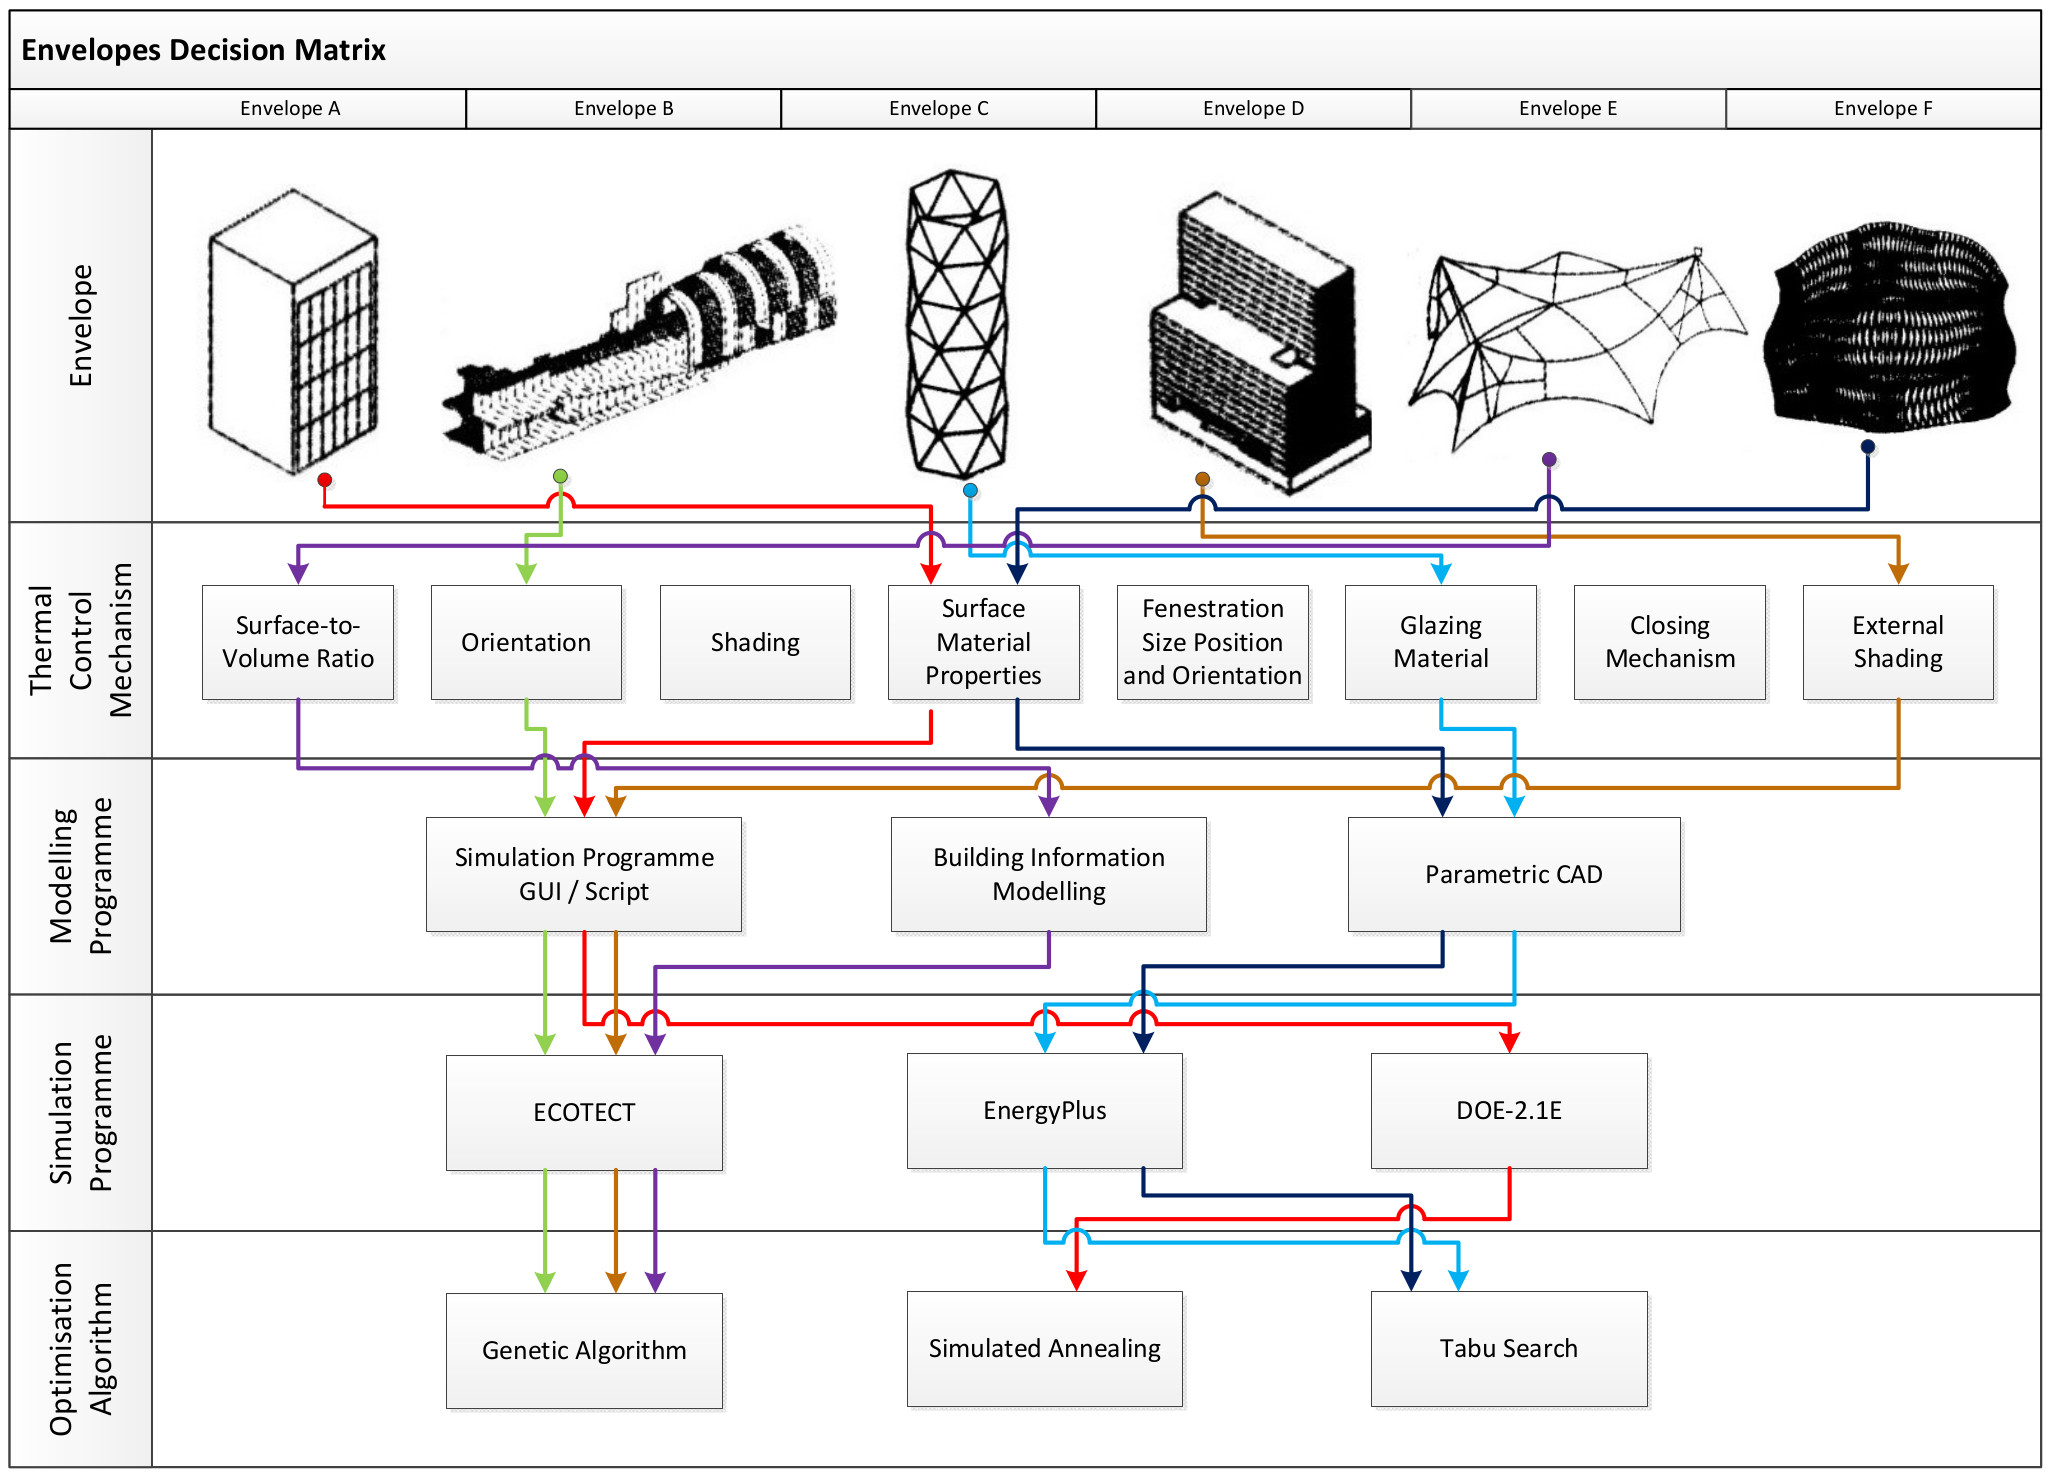
\includegraphics[width=19cm]{./Images/24-DecisionChart}
	\caption[Decision Flowchart]{Flowchart of decisions for each envelope example}
	\label{fig:DecisionChart}
\end{sidewaysfigure}

\clearpage
\section{Conclusions}

At this point, a systematical approach has been presented to assist the architect in his endeavour to create thermally efficient design of building envelopes using solar passive techniques throgh the utilisation of computer algorithm and simmulation programmes.

The conclusions from this study are:
\begin{enumerate}
	\item The computer algorithm is simply a programme designed by humans but operated by the computer, which means that it is subject to the computer's logic. This requires that the users input be planned very carefully to ensure logical and usefull results.
	\item In order to provide the right input and receive the desired outcome, the process of design using algorithm has been divided into four separate and consequtive stages:
		\begin{enumerate}
			\item \textbf{Analysis of Envelope Form}: the architect has to create a basic envelope form that responds to the basic requirements of the user as a basis for the optimisation process. The form must be analysed and categorised geometrically and in terms of architectural features, so that the architect may choose the fittest thermal control technique.
			\item \textbf{Design Intent: Thermal Criteria and Target Performance}: in this stage, according to envelope design and category, the architect chooses the control technique which would have the most significant effect on thermal performance. In addition, the architect must decide on the target performance according to internal space functions and needs.
			\item \textbf{Virtual Modelling and Simulation}: choosing the right tools for the creating of a parametric model, and the simulation of its thermal performance. This is mainly influenced by the chosen control techniques, as different simulation programmes have different features, strengths and weaknesses according to the function needed. Also, this stage is very important in future decisions concerning the programming method of the algorithm.
			\item \textbf{Programming and Optimisation}: the choice of modelling and simulation programmes is a crucial factor when deciding on the programming method. The optimisation algorithm is chosen based on the envelope form and the chosen thermal criteria and control techniques. Different algorithms have different search methods that may or may not be the best for the task. Finally the system is initiated and results are received.
		\end{enumerate}
	\item The study presented herein is general approach with regards to building types and forms, which aims at providing a systematic approach for thermal design of any building envelope. However, it lacks the practical details and problems of specific cases with a much more developed architectural design, which is the subject of future study.
	\item This approach helps the architect by minimising the amount of human error or misjudgment at the early stages of conceptual design. However, it is still subject to potential misjudgment by the user at stages 1 and 2, which is a subject for future study.
\end{enumerate}

